\section{Messwerte und Auswertung} % (fold)
\label{sec:messwerte_und_auswertung}

	\subsection{Bestimmung des Ausleserauschens} % (fold)
	\label{sub:bestimmung_des_ausleserauschens}
	
		Zur Bestimmung des systematischen Fehlers und des Rauschens mussten mehrere Biasbilder aufgenommen werden.
		Abbildung \ref{fig:beispiel-biasbild} zeigt ein Beispiel eines solchen Biasbildes, wie es von uns verwendet wurde.

		\begin{figure}
			\center
			\fbox{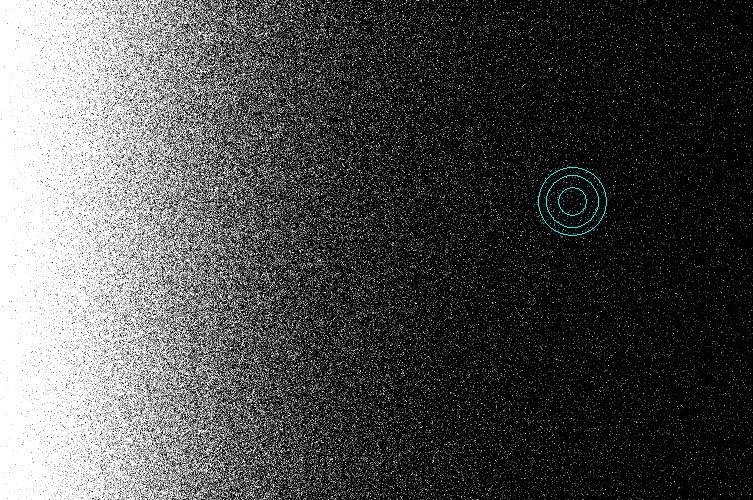
\includegraphics[scale=0.5]{messwerte/bias-1.jpg}}
			\caption{Beispiel einer Biasaufnahme bei $-8\unit{$^\circ$C}$ mit eingefügtem Messcursor}
			\label{fig:beispiel-biasbild}
		\end{figure}

		Für den weiteren Versuchsteil wurden genau 100 Biasbilder aufgenommen.
		Über diese Bilder wurde für jeden Pixel der Mittelwert gebildet, sodass ein Mittelwertbild entstand.
		Dieses ist in Abbildung \ref{fig:bias-mean} gezeigt.
		Es wird deutlich, dass sich der systematische Fehler entlang der Abzisse verändert.
		Durch Abzug dieses Bildes von anderen Aufnahmen kann der Einfluss des systematischen Fehlers bei Messungen näherungsweise als Null angenommen werden. 

		\begin{figure}
			\center
			\fbox{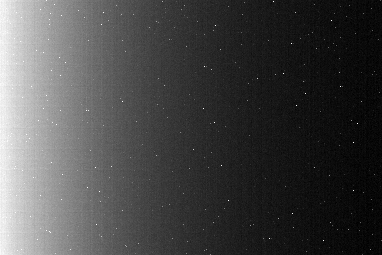
\includegraphics{messwerte/bias-mean.png}}
			\caption{Mittelwertbild von 100 aufgenommenen Biasbildern bei Raumtemperatur}
			\label{fig:bias-mean}
		\end{figure}

		Um ein Maß für den Wert des Rauschens zu erhalten, wurde nun noch ein weiteres Biasbild aufgenommen.
		Von dieser Aufnahme wurde das Mittelwertbild abgezogen.
		Da so diverse Pixel durchaus auch negative Werte annehmen könnten, wurde eine bekannten Konstante (auch Offset) von 200 hinzuaddiert. 
		Dieses Verfahren wurde auch für alle weiteren Differenzbilder, von denen zum Beispiel der systematische Fehler subtrahiert wurde, verwendet.
		Das erhaltene Rauschbild ist in Abbildung \ref{fig:bias-noise} gezeigt.

		\begin{figure}
			\center
			\fbox{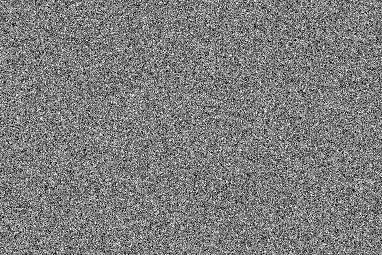
\includegraphics{messwerte/bias-noise.png}}
			\caption{Rauschbild bei Raumtemperatur mit Offset von 200}
			\label{fig:bias-noise}
		\end{figure}

		Die minimale Standardabweichung wurde über das Programm und mit Hilfe des Messcursors zu circa 11.2 bestimmt.
		Da uns in diesem Versuch aber mehr die Lage der Peaks im Spektrum als ihre Intensität interessiert, ist dieser Wert für die weitere Auswertung eher unerheblich.
		Im folgenden werden alle weiteren Aufnahmen auch immer, wenn nicht ausdrücklich anderes gesagt, nach Abzug des entsprechenden Biaslevels gezeigt und ausgewertet.

	% subsection bestimmung_des_ausleserauschens (end)


	\subsection{Temperaturabhängigkeit des Dunkelstromes} % (fold)
	\label{sub:temperaturabh_ngigkeit_des_dunkelstromes}

		Die Dunkelstrombilder wurden wie unter \ref{sub:dunkelstromaufnahme} gezeigt erstellt und im Anschluss wurde stets eine Bias-Aufnahme abgezogen.
		Als Beispiel sind in den Abbidungen \ref{dark04} und \ref{dark04_spec} die Intensitätsverteilungen des reduzierten Dunkelstrombildes bei $2\unit{$^\circ$C}$ zu sehen.
		Alle folgenden Dunkelstrombilder wurden mit einer Belichtungszeit von $5\unit{min}$ aufgenommen.

		\begin{figure}
			\center
			\fbox{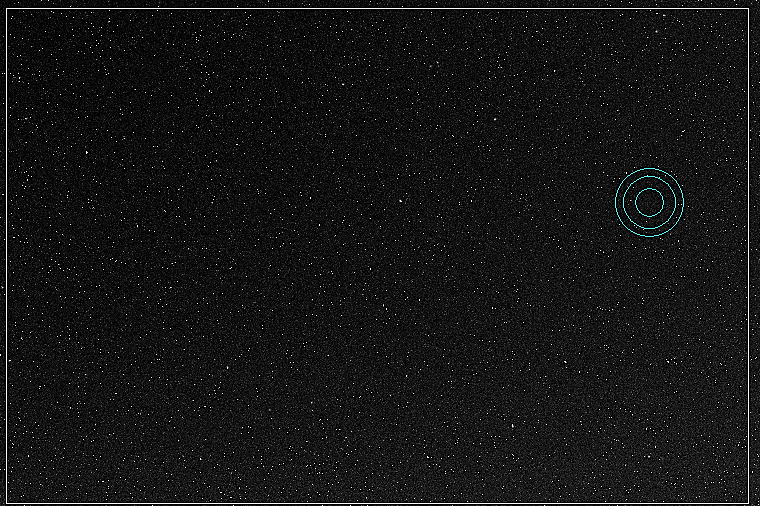
\includegraphics[scale=0.5]{messwerte/dark04.PNG}}
			\caption{Dunkelstrombild bei geschlossener Blende und $2\unit{$^\circ$C}$}
			\label{dark04}
		\end{figure}

		\begin{figure}
			\center
			% GNUPLOT: LaTeX picture with Postscript
\begingroup
  \makeatletter
  \providecommand\color[2][]{%
    \GenericError{(gnuplot) \space\space\space\@spaces}{%
      Package color not loaded in conjunction with
      terminal option `colourtext'%
    }{See the gnuplot documentation for explanation.%
    }{Either use 'blacktext' in gnuplot or load the package
      color.sty in LaTeX.}%
    \renewcommand\color[2][]{}%
  }%
  \providecommand\includegraphics[2][]{%
    \GenericError{(gnuplot) \space\space\space\@spaces}{%
      Package graphicx or graphics not loaded%
    }{See the gnuplot documentation for explanation.%
    }{The gnuplot epslatex terminal needs graphicx.sty or graphics.sty.}%
    \renewcommand\includegraphics[2][]{}%
  }%
  \providecommand\rotatebox[2]{#2}%
  \@ifundefined{ifGPcolor}{%
    \newif\ifGPcolor
    \GPcolorfalse
  }{}%
  \@ifundefined{ifGPblacktext}{%
    \newif\ifGPblacktext
    \GPblacktexttrue
  }{}%
  % define a \g@addto@macro without @ in the name:
  \let\gplgaddtomacro\g@addto@macro
  % define empty templates for all commands taking text:
  \gdef\gplbacktext{}%
  \gdef\gplfronttext{}%
  \makeatother
  \ifGPblacktext
    % no textcolor at all
    \def\colorrgb#1{}%
    \def\colorgray#1{}%
  \else
    % gray or color?
    \ifGPcolor
      \def\colorrgb#1{\color[rgb]{#1}}%
      \def\colorgray#1{\color[gray]{#1}}%
      \expandafter\def\csname LTw\endcsname{\color{white}}%
      \expandafter\def\csname LTb\endcsname{\color{black}}%
      \expandafter\def\csname LTa\endcsname{\color{black}}%
      \expandafter\def\csname LT0\endcsname{\color[rgb]{1,0,0}}%
      \expandafter\def\csname LT1\endcsname{\color[rgb]{0,1,0}}%
      \expandafter\def\csname LT2\endcsname{\color[rgb]{0,0,1}}%
      \expandafter\def\csname LT3\endcsname{\color[rgb]{1,0,1}}%
      \expandafter\def\csname LT4\endcsname{\color[rgb]{0,1,1}}%
      \expandafter\def\csname LT5\endcsname{\color[rgb]{1,1,0}}%
      \expandafter\def\csname LT6\endcsname{\color[rgb]{0,0,0}}%
      \expandafter\def\csname LT7\endcsname{\color[rgb]{1,0.3,0}}%
      \expandafter\def\csname LT8\endcsname{\color[rgb]{0.5,0.5,0.5}}%
    \else
      % gray
      \def\colorrgb#1{\color{black}}%
      \def\colorgray#1{\color[gray]{#1}}%
      \expandafter\def\csname LTw\endcsname{\color{white}}%
      \expandafter\def\csname LTb\endcsname{\color{black}}%
      \expandafter\def\csname LTa\endcsname{\color{black}}%
      \expandafter\def\csname LT0\endcsname{\color{black}}%
      \expandafter\def\csname LT1\endcsname{\color{black}}%
      \expandafter\def\csname LT2\endcsname{\color{black}}%
      \expandafter\def\csname LT3\endcsname{\color{black}}%
      \expandafter\def\csname LT4\endcsname{\color{black}}%
      \expandafter\def\csname LT5\endcsname{\color{black}}%
      \expandafter\def\csname LT6\endcsname{\color{black}}%
      \expandafter\def\csname LT7\endcsname{\color{black}}%
      \expandafter\def\csname LT8\endcsname{\color{black}}%
    \fi
  \fi
  \setlength{\unitlength}{0.0500bp}%
  \begin{picture}(6802.00,3968.00)%
    \gplgaddtomacro\gplbacktext{%
      \csname LTb\endcsname%
      \put(946,704){\makebox(0,0)[r]{\strut{} 300}}%
      \put(946,1132){\makebox(0,0)[r]{\strut{} 320}}%
      \put(946,1561){\makebox(0,0)[r]{\strut{} 340}}%
      \put(946,1989){\makebox(0,0)[r]{\strut{} 360}}%
      \put(946,2418){\makebox(0,0)[r]{\strut{} 380}}%
      \put(946,2846){\makebox(0,0)[r]{\strut{} 400}}%
      \put(946,3275){\makebox(0,0)[r]{\strut{} 420}}%
      \put(946,3703){\makebox(0,0)[r]{\strut{} 440}}%
      \put(1078,484){\makebox(0,0){\strut{} 0}}%
      \put(1744,484){\makebox(0,0){\strut{} 100}}%
      \put(2410,484){\makebox(0,0){\strut{} 200}}%
      \put(3076,484){\makebox(0,0){\strut{} 300}}%
      \put(3742,484){\makebox(0,0){\strut{} 400}}%
      \put(4407,484){\makebox(0,0){\strut{} 500}}%
      \put(5073,484){\makebox(0,0){\strut{} 600}}%
      \put(5739,484){\makebox(0,0){\strut{} 700}}%
      \put(6405,484){\makebox(0,0){\strut{} 800}}%
      \put(176,2203){\rotatebox{-270}{\makebox(0,0){\strut{}Intensität (willkürliche Einheit)}}}%
      \put(3741,154){\makebox(0,0){\strut{}Pixel}}%
    }%
    \gplgaddtomacro\gplfronttext{%
      \csname LTb\endcsname%
      \put(5418,3530){\makebox(0,0)[r]{\strut{}Messwerte}}%
    }%
    \gplbacktext
    \put(0,0){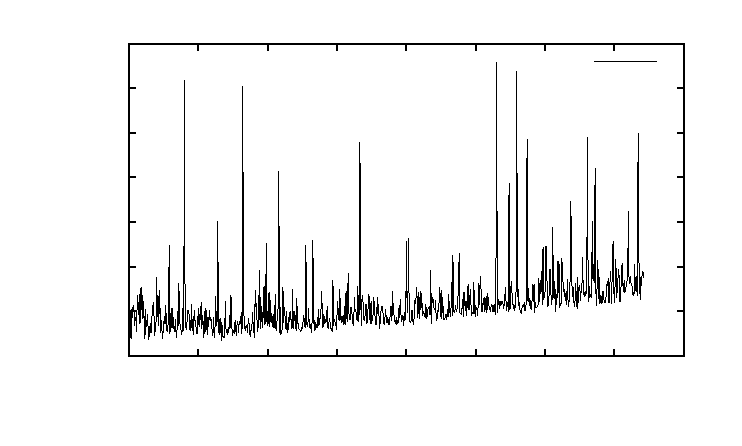
\includegraphics{dark04-spec}}%
    \gplfronttext
  \end{picture}%
\endgroup

			\caption{Signalverteilung über die Pixelspalten bei geschlossener Blende und $2\unit{$^\circ$C}$}
			\label{dark04_spec}
		\end{figure}

		Alle Signalverteilungen mitteln das Signal über eine Spalte von Pixeln und stellen es dann in Abhängigkeit des Spaltenindex dar.
		Zu erkennen ist klar ein Grundlevel um 320 und einzelne zufällige Spitzen.
		Diese können durch Temperaturveränderungen während der Aufnahme oder durch durchdringende Strahlung (natürliche Radioaktivität, kosmische Strahlung, etc.) entstanden sein.
		Trägt man nun die jeweiligen gemittelten Grundlevel der einzelnen Aufnahmen über der Temperatur auf, so ergibt sich der in Abbildung \ref{fig:dark-temp} gezeigte Zusammenhang:

		\begin{figure}
			\center
			% GNUPLOT: LaTeX picture with Postscript
\begingroup
  \makeatletter
  \providecommand\color[2][]{%
    \GenericError{(gnuplot) \space\space\space\@spaces}{%
      Package color not loaded in conjunction with
      terminal option `colourtext'%
    }{See the gnuplot documentation for explanation.%
    }{Either use 'blacktext' in gnuplot or load the package
      color.sty in LaTeX.}%
    \renewcommand\color[2][]{}%
  }%
  \providecommand\includegraphics[2][]{%
    \GenericError{(gnuplot) \space\space\space\@spaces}{%
      Package graphicx or graphics not loaded%
    }{See the gnuplot documentation for explanation.%
    }{The gnuplot epslatex terminal needs graphicx.sty or graphics.sty.}%
    \renewcommand\includegraphics[2][]{}%
  }%
  \providecommand\rotatebox[2]{#2}%
  \@ifundefined{ifGPcolor}{%
    \newif\ifGPcolor
    \GPcolorfalse
  }{}%
  \@ifundefined{ifGPblacktext}{%
    \newif\ifGPblacktext
    \GPblacktexttrue
  }{}%
  % define a \g@addto@macro without @ in the name:
  \let\gplgaddtomacro\g@addto@macro
  % define empty templates for all commands taking text:
  \gdef\gplbacktext{}%
  \gdef\gplfronttext{}%
  \makeatother
  \ifGPblacktext
    % no textcolor at all
    \def\colorrgb#1{}%
    \def\colorgray#1{}%
  \else
    % gray or color?
    \ifGPcolor
      \def\colorrgb#1{\color[rgb]{#1}}%
      \def\colorgray#1{\color[gray]{#1}}%
      \expandafter\def\csname LTw\endcsname{\color{white}}%
      \expandafter\def\csname LTb\endcsname{\color{black}}%
      \expandafter\def\csname LTa\endcsname{\color{black}}%
      \expandafter\def\csname LT0\endcsname{\color[rgb]{1,0,0}}%
      \expandafter\def\csname LT1\endcsname{\color[rgb]{0,1,0}}%
      \expandafter\def\csname LT2\endcsname{\color[rgb]{0,0,1}}%
      \expandafter\def\csname LT3\endcsname{\color[rgb]{1,0,1}}%
      \expandafter\def\csname LT4\endcsname{\color[rgb]{0,1,1}}%
      \expandafter\def\csname LT5\endcsname{\color[rgb]{1,1,0}}%
      \expandafter\def\csname LT6\endcsname{\color[rgb]{0,0,0}}%
      \expandafter\def\csname LT7\endcsname{\color[rgb]{1,0.3,0}}%
      \expandafter\def\csname LT8\endcsname{\color[rgb]{0.5,0.5,0.5}}%
    \else
      % gray
      \def\colorrgb#1{\color{black}}%
      \def\colorgray#1{\color[gray]{#1}}%
      \expandafter\def\csname LTw\endcsname{\color{white}}%
      \expandafter\def\csname LTb\endcsname{\color{black}}%
      \expandafter\def\csname LTa\endcsname{\color{black}}%
      \expandafter\def\csname LT0\endcsname{\color{black}}%
      \expandafter\def\csname LT1\endcsname{\color{black}}%
      \expandafter\def\csname LT2\endcsname{\color{black}}%
      \expandafter\def\csname LT3\endcsname{\color{black}}%
      \expandafter\def\csname LT4\endcsname{\color{black}}%
      \expandafter\def\csname LT5\endcsname{\color{black}}%
      \expandafter\def\csname LT6\endcsname{\color{black}}%
      \expandafter\def\csname LT7\endcsname{\color{black}}%
      \expandafter\def\csname LT8\endcsname{\color{black}}%
    \fi
  \fi
  \setlength{\unitlength}{0.0500bp}%
  \begin{picture}(6802.00,3968.00)%
    \gplgaddtomacro\gplbacktext{%
      \csname LTb\endcsname%
      \put(946,704){\makebox(0,0)[r]{\strut{}$0.10$}}%
      \put(946,1304){\makebox(0,0)[r]{\strut{}$0.15$}}%
      \put(946,1904){\makebox(0,0)[r]{\strut{}$0.20$}}%
      \put(946,2503){\makebox(0,0)[r]{\strut{}$0.25$}}%
      \put(946,3103){\makebox(0,0)[r]{\strut{}$0.30$}}%
      \put(946,3703){\makebox(0,0)[r]{\strut{}$0.35$}}%
      \put(1078,484){\makebox(0,0){\strut{}-10}}%
      \put(1966,484){\makebox(0,0){\strut{}-5}}%
      \put(2854,484){\makebox(0,0){\strut{} 0}}%
      \put(3742,484){\makebox(0,0){\strut{} 5}}%
      \put(4629,484){\makebox(0,0){\strut{} 10}}%
      \put(5517,484){\makebox(0,0){\strut{} 15}}%
      \put(6405,484){\makebox(0,0){\strut{} 20}}%
      \put(176,2203){\rotatebox{-270}{\makebox(0,0){\strut{}$1/\ln(I)$}}}%
      \put(3741,154){\makebox(0,0){\strut{}Temperatur $\vartheta\ [^\circ\mathrm{C}]$}}%
    }%
    \gplgaddtomacro\gplfronttext{%
      \csname LTb\endcsname%
      \put(5418,3530){\makebox(0,0)[r]{\strut{}Messwerte}}%
      \csname LTb\endcsname%
      \put(5418,3310){\makebox(0,0)[r]{\strut{}$f(\vartheta) = a\vartheta+b$}}%
    }%
    \gplbacktext
    \put(0,0){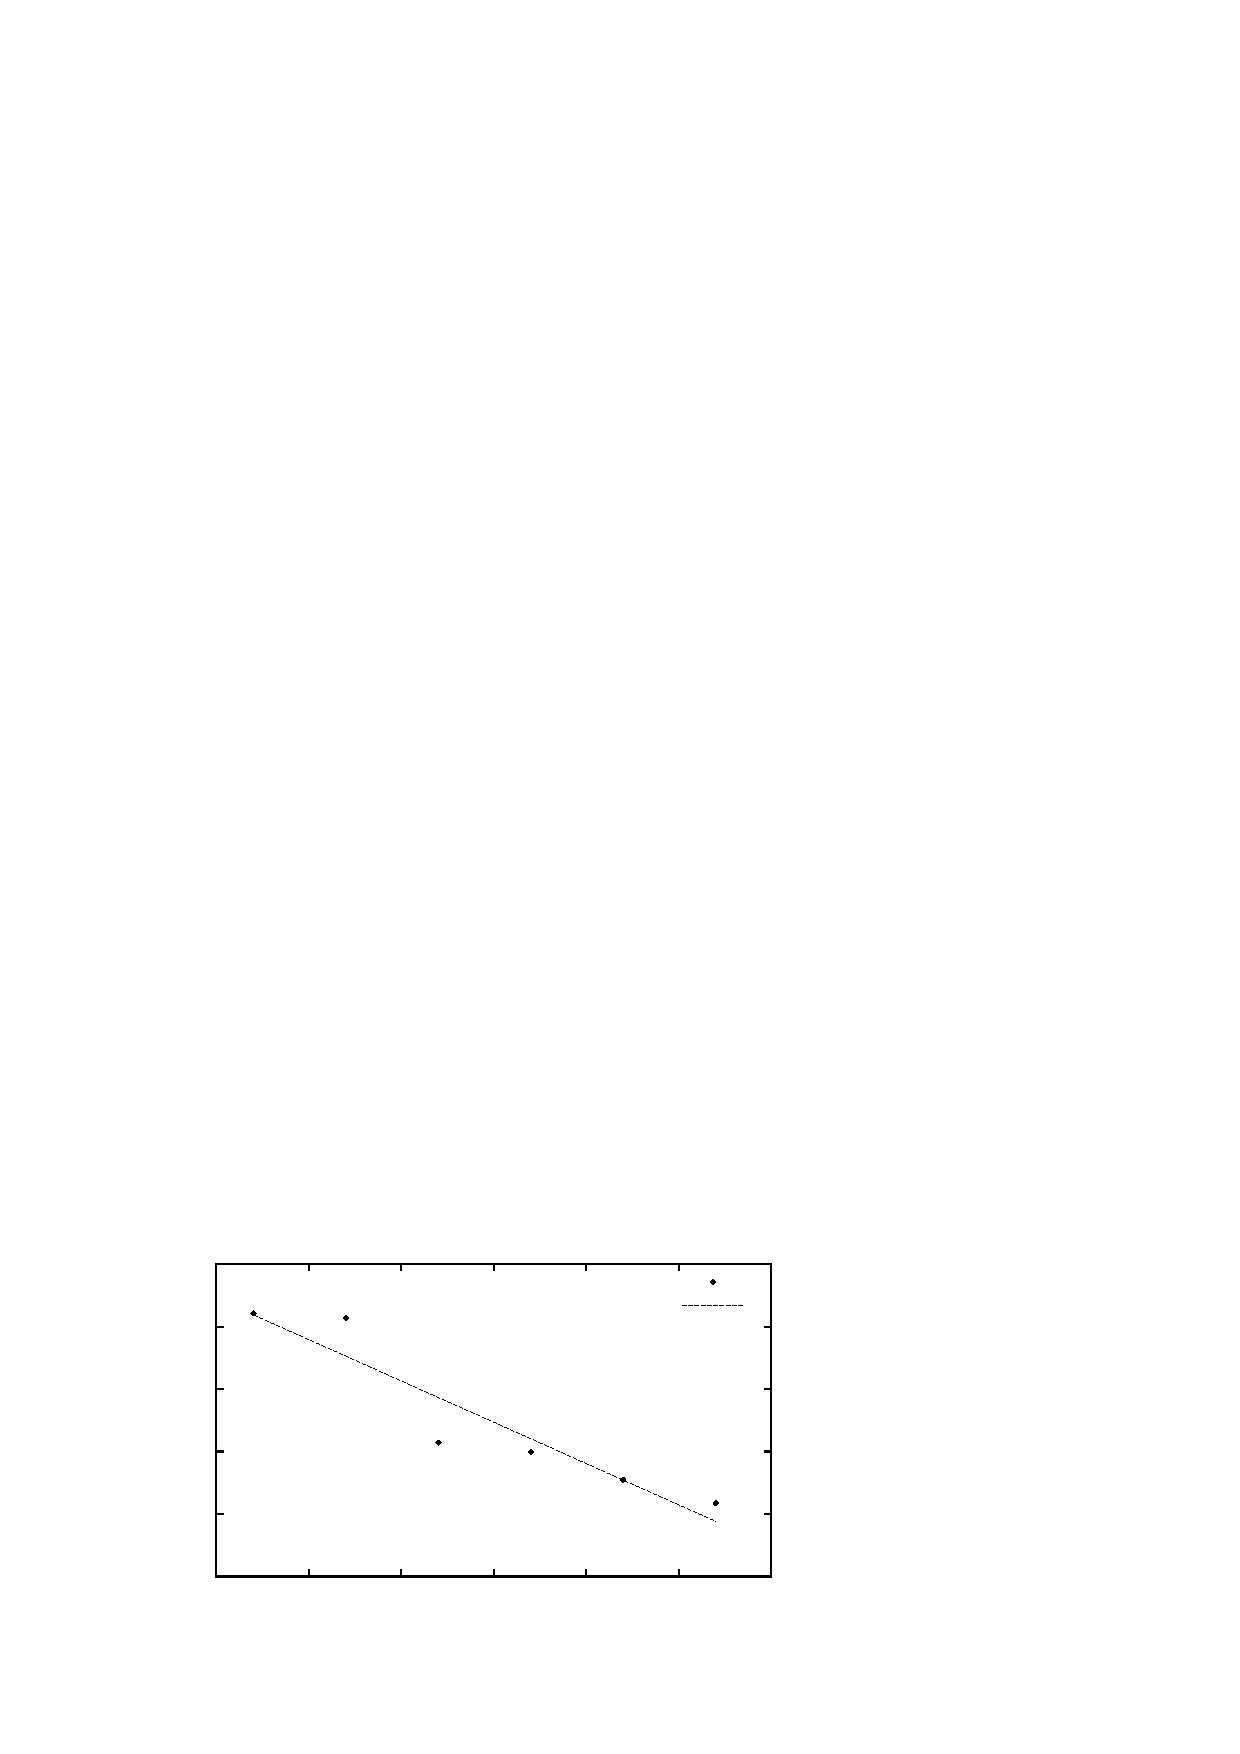
\includegraphics{dark-temp}}%
    \gplfronttext
  \end{picture}%
\endgroup

			\caption{Abhängigkeit des Dunkelstroms von der Temperatur}
			\label{fig:dark-temp}
		\end{figure}

		Legt man für die Temperaturabhängigkeit des Signals den folgenden Zusammenhang zugrunde,
		\[ I \propto \exp\curvb{-\frac{E_G}{kT}} \]
		wobei $E_G$ für die Bandlückenenergie des dotierten Halbleiters steht, $k$ die Boltzmann-Konstante und $T$ die absolute Temperatur beschreibt, so kann man aus dem gemittelten Anstieg $a$ der Ausgleichsgeraden $E_G$ bestimmen.
		\[ E_G = -\frac{k}{a} \]
		Aus der Approximation erhielten wir
		\[ a = (-0.0066 \pm 0.0012)\unit{JK}^{-1} \]
		Durch $\Delta a$ ergibt sich für $E_G$ ein relativer Fehler von ungefähr $20\unit{\%}$.
		\[ E_G \approx 2.1\cdot 10^{-21}\unit{J} = 13\unit{meV} \]
		Dieser Wert liegt im Bereichen des für Germanium typischen Wertes.
		Er ist damit also plausibel.
	
	% subsection temperaturabh_ngigkeit_des_dunkelstromes (end)


	\subsection{Linearität der CCD-Kamera} % (fold)
	\label{sub:linearit_t_der_ccd_kamera}

		Zur Überprüfung der Linearität wurde wie unter \ref{sub:_berpr_fung_der_linearit_t} beschrieben vorgegangen.
		Die Temperatur wurde dabei konstant auf $0\unit{$^\circ$C}$ gehalten und Biasaufnahmen wurden stets abgezogen.
		In Abbildung \ref{linspec} ist eine Beispielaufnahme dargestellt.

		\begin{figure}
			\center
			% GNUPLOT: LaTeX picture with Postscript
\begingroup
  \makeatletter
  \providecommand\color[2][]{%
    \GenericError{(gnuplot) \space\space\space\@spaces}{%
      Package color not loaded in conjunction with
      terminal option `colourtext'%
    }{See the gnuplot documentation for explanation.%
    }{Either use 'blacktext' in gnuplot or load the package
      color.sty in LaTeX.}%
    \renewcommand\color[2][]{}%
  }%
  \providecommand\includegraphics[2][]{%
    \GenericError{(gnuplot) \space\space\space\@spaces}{%
      Package graphicx or graphics not loaded%
    }{See the gnuplot documentation for explanation.%
    }{The gnuplot epslatex terminal needs graphicx.sty or graphics.sty.}%
    \renewcommand\includegraphics[2][]{}%
  }%
  \providecommand\rotatebox[2]{#2}%
  \@ifundefined{ifGPcolor}{%
    \newif\ifGPcolor
    \GPcolorfalse
  }{}%
  \@ifundefined{ifGPblacktext}{%
    \newif\ifGPblacktext
    \GPblacktexttrue
  }{}%
  % define a \g@addto@macro without @ in the name:
  \let\gplgaddtomacro\g@addto@macro
  % define empty templates for all commands taking text:
  \gdef\gplbacktext{}%
  \gdef\gplfronttext{}%
  \makeatother
  \ifGPblacktext
    % no textcolor at all
    \def\colorrgb#1{}%
    \def\colorgray#1{}%
  \else
    % gray or color?
    \ifGPcolor
      \def\colorrgb#1{\color[rgb]{#1}}%
      \def\colorgray#1{\color[gray]{#1}}%
      \expandafter\def\csname LTw\endcsname{\color{white}}%
      \expandafter\def\csname LTb\endcsname{\color{black}}%
      \expandafter\def\csname LTa\endcsname{\color{black}}%
      \expandafter\def\csname LT0\endcsname{\color[rgb]{1,0,0}}%
      \expandafter\def\csname LT1\endcsname{\color[rgb]{0,1,0}}%
      \expandafter\def\csname LT2\endcsname{\color[rgb]{0,0,1}}%
      \expandafter\def\csname LT3\endcsname{\color[rgb]{1,0,1}}%
      \expandafter\def\csname LT4\endcsname{\color[rgb]{0,1,1}}%
      \expandafter\def\csname LT5\endcsname{\color[rgb]{1,1,0}}%
      \expandafter\def\csname LT6\endcsname{\color[rgb]{0,0,0}}%
      \expandafter\def\csname LT7\endcsname{\color[rgb]{1,0.3,0}}%
      \expandafter\def\csname LT8\endcsname{\color[rgb]{0.5,0.5,0.5}}%
    \else
      % gray
      \def\colorrgb#1{\color{black}}%
      \def\colorgray#1{\color[gray]{#1}}%
      \expandafter\def\csname LTw\endcsname{\color{white}}%
      \expandafter\def\csname LTb\endcsname{\color{black}}%
      \expandafter\def\csname LTa\endcsname{\color{black}}%
      \expandafter\def\csname LT0\endcsname{\color{black}}%
      \expandafter\def\csname LT1\endcsname{\color{black}}%
      \expandafter\def\csname LT2\endcsname{\color{black}}%
      \expandafter\def\csname LT3\endcsname{\color{black}}%
      \expandafter\def\csname LT4\endcsname{\color{black}}%
      \expandafter\def\csname LT5\endcsname{\color{black}}%
      \expandafter\def\csname LT6\endcsname{\color{black}}%
      \expandafter\def\csname LT7\endcsname{\color{black}}%
      \expandafter\def\csname LT8\endcsname{\color{black}}%
    \fi
  \fi
  \setlength{\unitlength}{0.0500bp}%
  \begin{picture}(6802.00,3968.00)%
    \gplgaddtomacro\gplbacktext{%
      \csname LTb\endcsname%
      \put(1078,704){\makebox(0,0)[r]{\strut{} 1100}}%
      \put(1078,1304){\makebox(0,0)[r]{\strut{} 1200}}%
      \put(1078,1904){\makebox(0,0)[r]{\strut{} 1300}}%
      \put(1078,2503){\makebox(0,0)[r]{\strut{} 1400}}%
      \put(1078,3103){\makebox(0,0)[r]{\strut{} 1500}}%
      \put(1078,3703){\makebox(0,0)[r]{\strut{} 1600}}%
      \put(1210,484){\makebox(0,0){\strut{} 0}}%
      \put(1859,484){\makebox(0,0){\strut{} 100}}%
      \put(2509,484){\makebox(0,0){\strut{} 200}}%
      \put(3158,484){\makebox(0,0){\strut{} 300}}%
      \put(3808,484){\makebox(0,0){\strut{} 400}}%
      \put(4457,484){\makebox(0,0){\strut{} 500}}%
      \put(5106,484){\makebox(0,0){\strut{} 600}}%
      \put(5756,484){\makebox(0,0){\strut{} 700}}%
      \put(6405,484){\makebox(0,0){\strut{} 800}}%
      \put(176,2203){\rotatebox{-270}{\makebox(0,0){\strut{}Intensität (willkürliche Einheit)}}}%
      \put(3807,154){\makebox(0,0){\strut{}Pixel}}%
    }%
    \gplgaddtomacro\gplfronttext{%
      \csname LTb\endcsname%
      \put(5418,3530){\makebox(0,0)[r]{\strut{}Messwerte}}%
    }%
    \gplbacktext
    \put(0,0){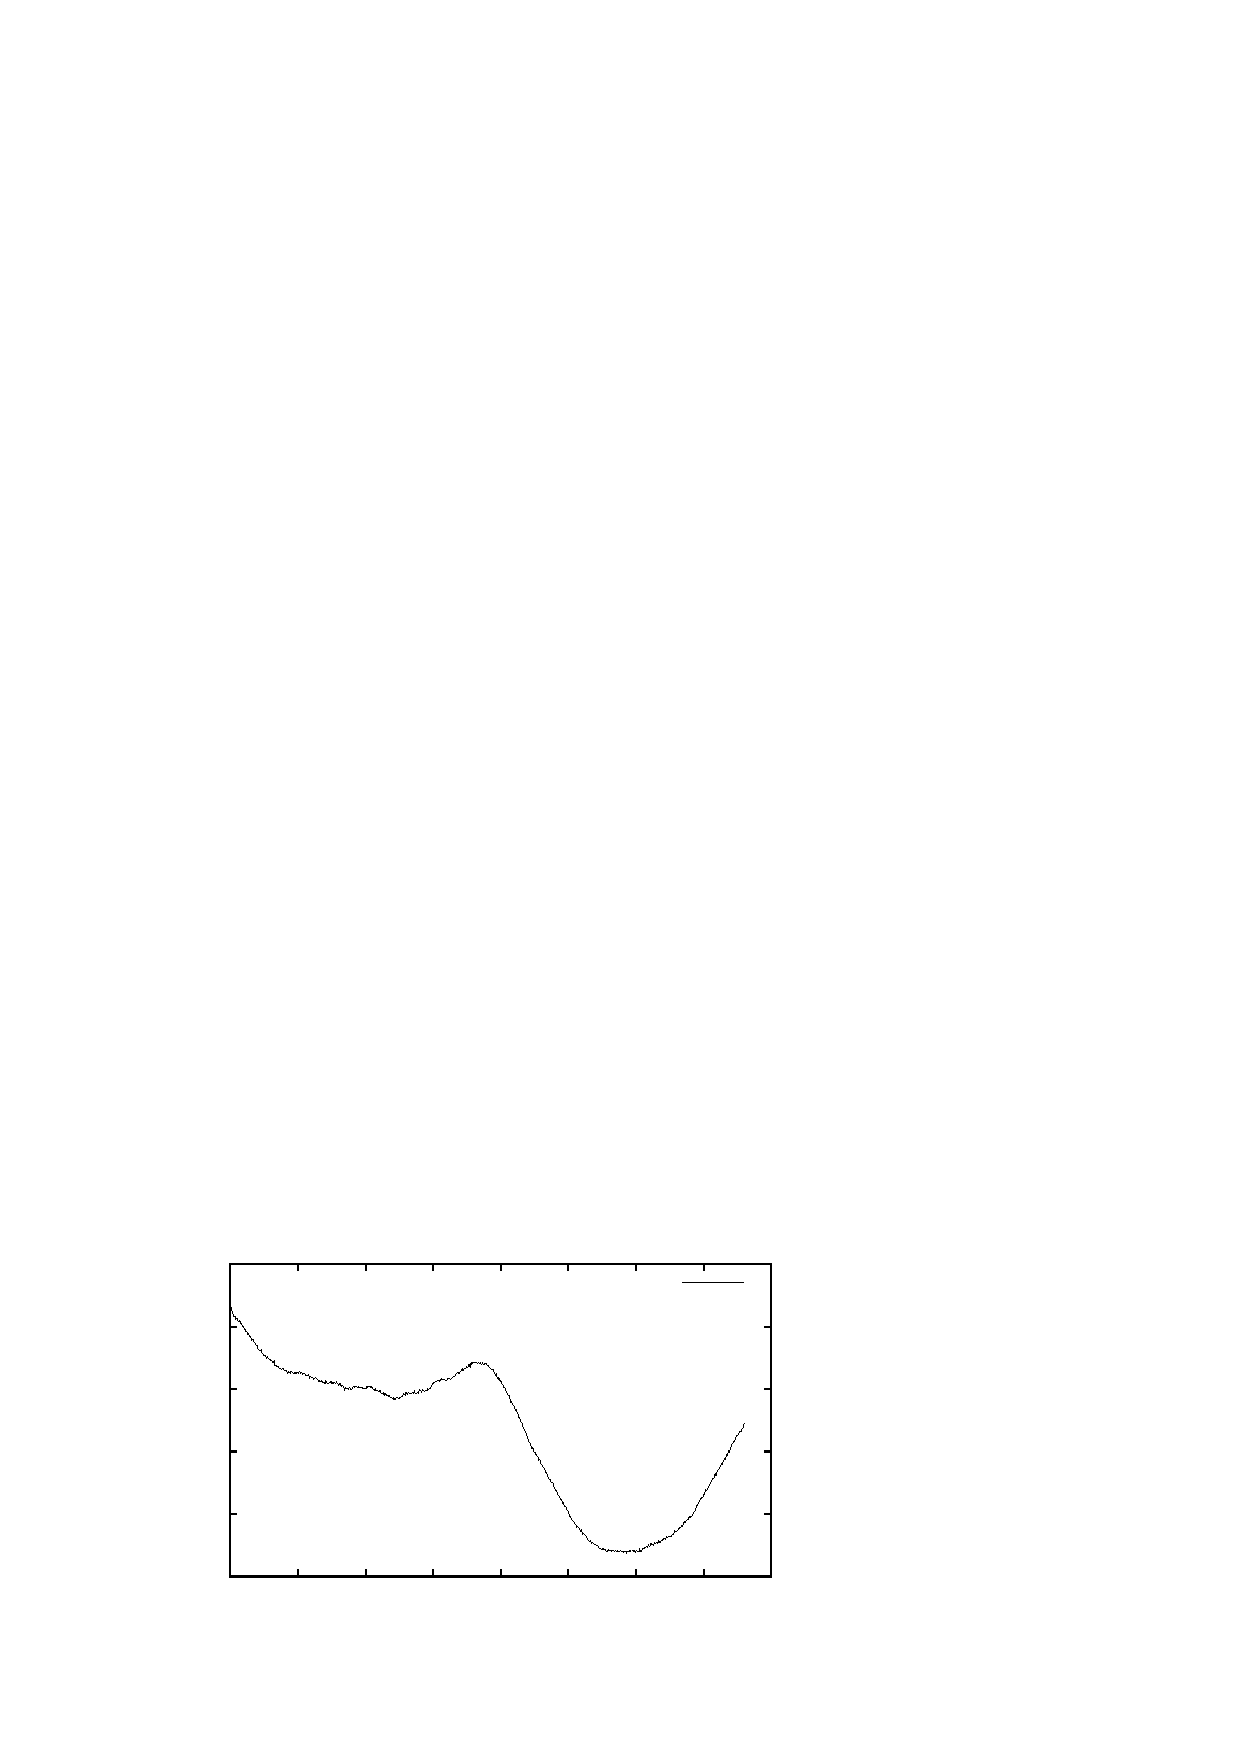
\includegraphics{linearspec}}%
    \gplfronttext
  \end{picture}%
\endgroup

			\caption{CCD-Aufnahme bei Beleuchtung mit Mikroskoplampe und vorgesetzter Lochblende, gemessen bei $0\unit{$^\circ$C}$, Belichtungszeit 0.5s}
			\label{linspec}
		\end{figure}

		Im Weiteren Vorgehen wurde stets das mittlere Maximum als Bezugspunkt gewählt.
		Da alle Aufnahmen unabhängig von der Belichtungszeit den gleichen (qualitativen) Verlauf aufwiesen, ist es völlig ausreichend nur die Werte an diesem Punkt zu untersuchen.
		Die jeweiligen Intensitätswerte am Maximum wurden über der Belichtungszeit in Abbildung \ref{linrise} zusammengefasst.

		\begin{figure}
			\center
			% GNUPLOT: LaTeX picture with Postscript
\begingroup
  \makeatletter
  \providecommand\color[2][]{%
    \GenericError{(gnuplot) \space\space\space\@spaces}{%
      Package color not loaded in conjunction with
      terminal option `colourtext'%
    }{See the gnuplot documentation for explanation.%
    }{Either use 'blacktext' in gnuplot or load the package
      color.sty in LaTeX.}%
    \renewcommand\color[2][]{}%
  }%
  \providecommand\includegraphics[2][]{%
    \GenericError{(gnuplot) \space\space\space\@spaces}{%
      Package graphicx or graphics not loaded%
    }{See the gnuplot documentation for explanation.%
    }{The gnuplot epslatex terminal needs graphicx.sty or graphics.sty.}%
    \renewcommand\includegraphics[2][]{}%
  }%
  \providecommand\rotatebox[2]{#2}%
  \@ifundefined{ifGPcolor}{%
    \newif\ifGPcolor
    \GPcolorfalse
  }{}%
  \@ifundefined{ifGPblacktext}{%
    \newif\ifGPblacktext
    \GPblacktexttrue
  }{}%
  % define a \g@addto@macro without @ in the name:
  \let\gplgaddtomacro\g@addto@macro
  % define empty templates for all commands taking text:
  \gdef\gplbacktext{}%
  \gdef\gplfronttext{}%
  \makeatother
  \ifGPblacktext
    % no textcolor at all
    \def\colorrgb#1{}%
    \def\colorgray#1{}%
  \else
    % gray or color?
    \ifGPcolor
      \def\colorrgb#1{\color[rgb]{#1}}%
      \def\colorgray#1{\color[gray]{#1}}%
      \expandafter\def\csname LTw\endcsname{\color{white}}%
      \expandafter\def\csname LTb\endcsname{\color{black}}%
      \expandafter\def\csname LTa\endcsname{\color{black}}%
      \expandafter\def\csname LT0\endcsname{\color[rgb]{1,0,0}}%
      \expandafter\def\csname LT1\endcsname{\color[rgb]{0,1,0}}%
      \expandafter\def\csname LT2\endcsname{\color[rgb]{0,0,1}}%
      \expandafter\def\csname LT3\endcsname{\color[rgb]{1,0,1}}%
      \expandafter\def\csname LT4\endcsname{\color[rgb]{0,1,1}}%
      \expandafter\def\csname LT5\endcsname{\color[rgb]{1,1,0}}%
      \expandafter\def\csname LT6\endcsname{\color[rgb]{0,0,0}}%
      \expandafter\def\csname LT7\endcsname{\color[rgb]{1,0.3,0}}%
      \expandafter\def\csname LT8\endcsname{\color[rgb]{0.5,0.5,0.5}}%
    \else
      % gray
      \def\colorrgb#1{\color{black}}%
      \def\colorgray#1{\color[gray]{#1}}%
      \expandafter\def\csname LTw\endcsname{\color{white}}%
      \expandafter\def\csname LTb\endcsname{\color{black}}%
      \expandafter\def\csname LTa\endcsname{\color{black}}%
      \expandafter\def\csname LT0\endcsname{\color{black}}%
      \expandafter\def\csname LT1\endcsname{\color{black}}%
      \expandafter\def\csname LT2\endcsname{\color{black}}%
      \expandafter\def\csname LT3\endcsname{\color{black}}%
      \expandafter\def\csname LT4\endcsname{\color{black}}%
      \expandafter\def\csname LT5\endcsname{\color{black}}%
      \expandafter\def\csname LT6\endcsname{\color{black}}%
      \expandafter\def\csname LT7\endcsname{\color{black}}%
      \expandafter\def\csname LT8\endcsname{\color{black}}%
    \fi
  \fi
  \setlength{\unitlength}{0.0500bp}%
  \begin{picture}(6802.00,3968.00)%
    \gplgaddtomacro\gplbacktext{%
      \csname LTb\endcsname%
      \put(1210,704){\makebox(0,0)[r]{\strut{} 0}}%
      \put(1210,1132){\makebox(0,0)[r]{\strut{} 2000}}%
      \put(1210,1561){\makebox(0,0)[r]{\strut{} 4000}}%
      \put(1210,1989){\makebox(0,0)[r]{\strut{} 6000}}%
      \put(1210,2418){\makebox(0,0)[r]{\strut{} 8000}}%
      \put(1210,2846){\makebox(0,0)[r]{\strut{} 10000}}%
      \put(1210,3275){\makebox(0,0)[r]{\strut{} 12000}}%
      \put(1210,3703){\makebox(0,0)[r]{\strut{} 14000}}%
      \put(1342,484){\makebox(0,0){\strut{} 0}}%
      \put(1848,484){\makebox(0,0){\strut{} 0.5}}%
      \put(2355,484){\makebox(0,0){\strut{} 1}}%
      \put(2861,484){\makebox(0,0){\strut{} 1.5}}%
      \put(3367,484){\makebox(0,0){\strut{} 2}}%
      \put(3874,484){\makebox(0,0){\strut{} 2.5}}%
      \put(4380,484){\makebox(0,0){\strut{} 3}}%
      \put(4886,484){\makebox(0,0){\strut{} 3.5}}%
      \put(5392,484){\makebox(0,0){\strut{} 4}}%
      \put(5899,484){\makebox(0,0){\strut{} 4.5}}%
      \put(6405,484){\makebox(0,0){\strut{} 5}}%
      \put(176,2203){\rotatebox{-270}{\makebox(0,0){\strut{}Intensität (willkürliche Einheit)}}}%
      \put(3873,154){\makebox(0,0){\strut{}Belichtungszeit in Sekunden}}%
    }%
    \gplgaddtomacro\gplfronttext{%
      \csname LTb\endcsname%
      \put(5418,3530){\makebox(0,0)[r]{\strut{}Messwerte}}%
    }%
    \gplbacktext
    \put(0,0){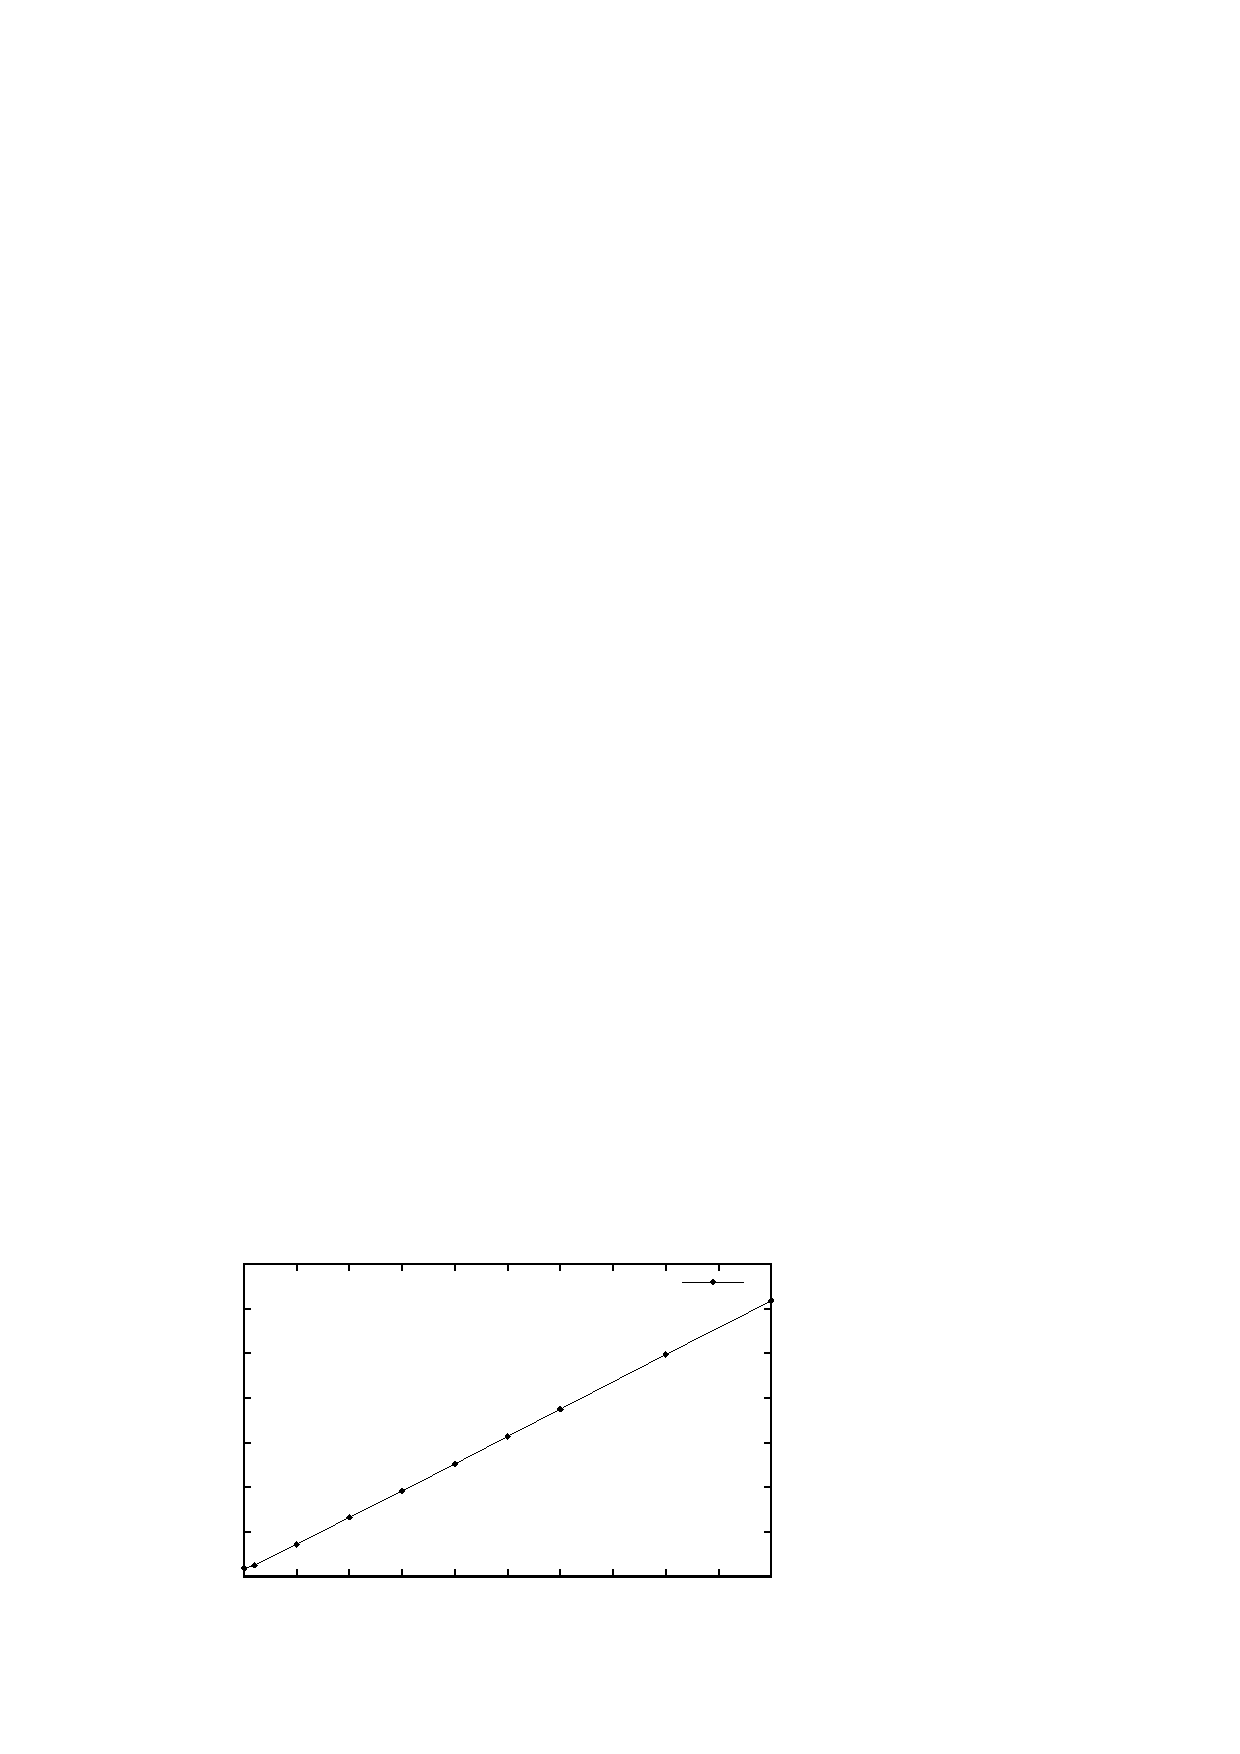
\includegraphics{linrise}}%
    \gplfronttext
  \end{picture}%
\endgroup

			\caption{CCD-Signal am mittleren Peak in Abhängigkeit der Belichtungszeit, gemessen bei $0\unit{$^\circ$C}$, Maximum mit Hilfe von Gnuplot ausgemessen}
			%stimmt nicht, es war mit Hilfe von Scidavis, muhahah!
			\label{linrise}
		\end{figure}

		Die lineare Anstiegsgerade ist offensichtlich und bestätigt in sehr guter Weise die Annahme und Forderung, dass die CCD-Zellen Elektronen proportional zur eingestrahlten Energie ansammeln.
		Der minimale Knick und das Offset um den Nullpunkt wird plausibel, wenn man den endlichen Dunkelstrom bedenkt und vor allem das stets aufaddierte Offset von 200 mit einbezieht.
		Abbildung \ref{linrise} zeigt somit eindeutig, dass die CCD über einen sehr weiten Bereich linear arbeitet und somit für unsere Zwecke bestens geeignet ist.

	% subsection linearit_t_der_ccd_kamera (end)


	\subsection{Vergleichsspektren von Hg-Cd und Ne} % (fold)
	\label{sub:vergleichsspektren_von_hg_cd_und_ne}

		Zur Kalibrierung und zum besseren Verständnis der Arbeitsweise des Gitterspektrografen wurden die Spektren einer Quecksilber-Cadmium-Entladungslampe sowie einer Neon-Glimmlampe aufgenommen, da diese gut zu erkennende und zuzuordnende Spektrallinien in unterschiedlichen Wellenlängenbereichen aufweisen.
		Da die Lampen erst zur Kalibrierung dienen, kann ihr Spektrum in diesem Abschnitt natürlich nur qualitativ ausgewertet werden.
		Die aufgenommenen Spektrallinien der Hg-Cd-Lampe sind in Abbildung \ref{hg_01} zu sehen. Weil das Licht der Lampe sehr intensiv war, wurde ein Papierfilter zwischen Optik und Lampe gebracht. 
		Dieser veränderte zwar durch sein Absorptionsverhalten die Intensität der Peaks jedoch nicht deren Lage.

		\begin{figure}
			\center
			% GNUPLOT: LaTeX picture with Postscript
\begingroup
  \makeatletter
  \providecommand\color[2][]{%
    \GenericError{(gnuplot) \space\space\space\@spaces}{%
      Package color not loaded in conjunction with
      terminal option `colourtext'%
    }{See the gnuplot documentation for explanation.%
    }{Either use 'blacktext' in gnuplot or load the package
      color.sty in LaTeX.}%
    \renewcommand\color[2][]{}%
  }%
  \providecommand\includegraphics[2][]{%
    \GenericError{(gnuplot) \space\space\space\@spaces}{%
      Package graphicx or graphics not loaded%
    }{See the gnuplot documentation for explanation.%
    }{The gnuplot epslatex terminal needs graphicx.sty or graphics.sty.}%
    \renewcommand\includegraphics[2][]{}%
  }%
  \providecommand\rotatebox[2]{#2}%
  \@ifundefined{ifGPcolor}{%
    \newif\ifGPcolor
    \GPcolorfalse
  }{}%
  \@ifundefined{ifGPblacktext}{%
    \newif\ifGPblacktext
    \GPblacktexttrue
  }{}%
  % define a \g@addto@macro without @ in the name:
  \let\gplgaddtomacro\g@addto@macro
  % define empty templates for all commands taking text:
  \gdef\gplbacktext{}%
  \gdef\gplfronttext{}%
  \makeatother
  \ifGPblacktext
    % no textcolor at all
    \def\colorrgb#1{}%
    \def\colorgray#1{}%
  \else
    % gray or color?
    \ifGPcolor
      \def\colorrgb#1{\color[rgb]{#1}}%
      \def\colorgray#1{\color[gray]{#1}}%
      \expandafter\def\csname LTw\endcsname{\color{white}}%
      \expandafter\def\csname LTb\endcsname{\color{black}}%
      \expandafter\def\csname LTa\endcsname{\color{black}}%
      \expandafter\def\csname LT0\endcsname{\color[rgb]{1,0,0}}%
      \expandafter\def\csname LT1\endcsname{\color[rgb]{0,1,0}}%
      \expandafter\def\csname LT2\endcsname{\color[rgb]{0,0,1}}%
      \expandafter\def\csname LT3\endcsname{\color[rgb]{1,0,1}}%
      \expandafter\def\csname LT4\endcsname{\color[rgb]{0,1,1}}%
      \expandafter\def\csname LT5\endcsname{\color[rgb]{1,1,0}}%
      \expandafter\def\csname LT6\endcsname{\color[rgb]{0,0,0}}%
      \expandafter\def\csname LT7\endcsname{\color[rgb]{1,0.3,0}}%
      \expandafter\def\csname LT8\endcsname{\color[rgb]{0.5,0.5,0.5}}%
    \else
      % gray
      \def\colorrgb#1{\color{black}}%
      \def\colorgray#1{\color[gray]{#1}}%
      \expandafter\def\csname LTw\endcsname{\color{white}}%
      \expandafter\def\csname LTb\endcsname{\color{black}}%
      \expandafter\def\csname LTa\endcsname{\color{black}}%
      \expandafter\def\csname LT0\endcsname{\color{black}}%
      \expandafter\def\csname LT1\endcsname{\color{black}}%
      \expandafter\def\csname LT2\endcsname{\color{black}}%
      \expandafter\def\csname LT3\endcsname{\color{black}}%
      \expandafter\def\csname LT4\endcsname{\color{black}}%
      \expandafter\def\csname LT5\endcsname{\color{black}}%
      \expandafter\def\csname LT6\endcsname{\color{black}}%
      \expandafter\def\csname LT7\endcsname{\color{black}}%
      \expandafter\def\csname LT8\endcsname{\color{black}}%
    \fi
  \fi
  \setlength{\unitlength}{0.0500bp}%
  \begin{picture}(6802.00,3968.00)%
    \gplgaddtomacro\gplbacktext{%
      \csname LTb\endcsname%
      \put(1078,704){\makebox(0,0)[r]{\strut{} 0}}%
      \put(1078,1132){\makebox(0,0)[r]{\strut{} 500}}%
      \put(1078,1561){\makebox(0,0)[r]{\strut{} 1000}}%
      \put(1078,1989){\makebox(0,0)[r]{\strut{} 1500}}%
      \put(1078,2418){\makebox(0,0)[r]{\strut{} 2000}}%
      \put(1078,2846){\makebox(0,0)[r]{\strut{} 2500}}%
      \put(1078,3275){\makebox(0,0)[r]{\strut{} 3000}}%
      \put(1078,3703){\makebox(0,0)[r]{\strut{} 3500}}%
      \put(1210,484){\makebox(0,0){\strut{} 0}}%
      \put(1859,484){\makebox(0,0){\strut{} 100}}%
      \put(2509,484){\makebox(0,0){\strut{} 200}}%
      \put(3158,484){\makebox(0,0){\strut{} 300}}%
      \put(3808,484){\makebox(0,0){\strut{} 400}}%
      \put(4457,484){\makebox(0,0){\strut{} 500}}%
      \put(5106,484){\makebox(0,0){\strut{} 600}}%
      \put(5756,484){\makebox(0,0){\strut{} 700}}%
      \put(6405,484){\makebox(0,0){\strut{} 800}}%
      \put(176,2203){\rotatebox{-270}{\makebox(0,0){\strut{}Intensität (willkürliche Einheit)}}}%
      \put(3807,154){\makebox(0,0){\strut{}Pixel}}%
    }%
    \gplgaddtomacro\gplfronttext{%
      \csname LTb\endcsname%
      \put(5418,3530){\makebox(0,0)[r]{\strut{}Messwerte}}%
    }%
    \gplbacktext
    \put(0,0){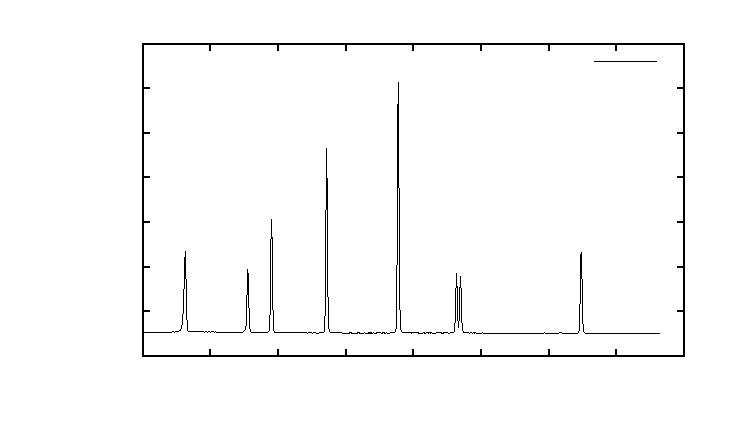
\includegraphics{hg-01}}%
    \gplfronttext
  \end{picture}%
\endgroup

			\caption{Spektrum der Quecksilber-Cadmium-Entladungslampe betrachtet durch die mittlere Blende bei verwendetem Gitter mit $g=200$, vorangestellten Papierfilter, Belichtungszeit von 0.1 s und Temperatur von $0\unit{$^\circ$C}$}
			\label{hg_01}
		\end{figure}

		Zu sehen sind alle charakteristischen Linien von Quecksilber und Cadmium von 405 bis $644\unit{nm}$ wie sie auch in der Referenz im Anhang \ref{sec:vergleichsspektren} zu finden sind.
		Die verminderte Intensität des Doppelpeaks und der Übrigen ist, wie oben erklärt, der Absorption des Papierfilters verschuldet.
		Wie wir sehen, reicht hier die Auflösung des groben Gitters vollkommen aus, um alle relevanten Linien zu zeigen und es bringt zu dem den Vorteil, das gesamte Spektrum auf eine Aufnahme zu projizieren.
		Nach Anpassung des Winkels an den Spektralbereich der Neon-Glimmlampe konnte das Bild von Abbildung \ref{ne_01} aufgenommen werden.

		\begin{figure}
			\center
			% GNUPLOT: LaTeX picture with Postscript
\begingroup
  \makeatletter
  \providecommand\color[2][]{%
    \GenericError{(gnuplot) \space\space\space\@spaces}{%
      Package color not loaded in conjunction with
      terminal option `colourtext'%
    }{See the gnuplot documentation for explanation.%
    }{Either use 'blacktext' in gnuplot or load the package
      color.sty in LaTeX.}%
    \renewcommand\color[2][]{}%
  }%
  \providecommand\includegraphics[2][]{%
    \GenericError{(gnuplot) \space\space\space\@spaces}{%
      Package graphicx or graphics not loaded%
    }{See the gnuplot documentation for explanation.%
    }{The gnuplot epslatex terminal needs graphicx.sty or graphics.sty.}%
    \renewcommand\includegraphics[2][]{}%
  }%
  \providecommand\rotatebox[2]{#2}%
  \@ifundefined{ifGPcolor}{%
    \newif\ifGPcolor
    \GPcolorfalse
  }{}%
  \@ifundefined{ifGPblacktext}{%
    \newif\ifGPblacktext
    \GPblacktexttrue
  }{}%
  % define a \g@addto@macro without @ in the name:
  \let\gplgaddtomacro\g@addto@macro
  % define empty templates for all commands taking text:
  \gdef\gplbacktext{}%
  \gdef\gplfronttext{}%
  \makeatother
  \ifGPblacktext
    % no textcolor at all
    \def\colorrgb#1{}%
    \def\colorgray#1{}%
  \else
    % gray or color?
    \ifGPcolor
      \def\colorrgb#1{\color[rgb]{#1}}%
      \def\colorgray#1{\color[gray]{#1}}%
      \expandafter\def\csname LTw\endcsname{\color{white}}%
      \expandafter\def\csname LTb\endcsname{\color{black}}%
      \expandafter\def\csname LTa\endcsname{\color{black}}%
      \expandafter\def\csname LT0\endcsname{\color[rgb]{1,0,0}}%
      \expandafter\def\csname LT1\endcsname{\color[rgb]{0,1,0}}%
      \expandafter\def\csname LT2\endcsname{\color[rgb]{0,0,1}}%
      \expandafter\def\csname LT3\endcsname{\color[rgb]{1,0,1}}%
      \expandafter\def\csname LT4\endcsname{\color[rgb]{0,1,1}}%
      \expandafter\def\csname LT5\endcsname{\color[rgb]{1,1,0}}%
      \expandafter\def\csname LT6\endcsname{\color[rgb]{0,0,0}}%
      \expandafter\def\csname LT7\endcsname{\color[rgb]{1,0.3,0}}%
      \expandafter\def\csname LT8\endcsname{\color[rgb]{0.5,0.5,0.5}}%
    \else
      % gray
      \def\colorrgb#1{\color{black}}%
      \def\colorgray#1{\color[gray]{#1}}%
      \expandafter\def\csname LTw\endcsname{\color{white}}%
      \expandafter\def\csname LTb\endcsname{\color{black}}%
      \expandafter\def\csname LTa\endcsname{\color{black}}%
      \expandafter\def\csname LT0\endcsname{\color{black}}%
      \expandafter\def\csname LT1\endcsname{\color{black}}%
      \expandafter\def\csname LT2\endcsname{\color{black}}%
      \expandafter\def\csname LT3\endcsname{\color{black}}%
      \expandafter\def\csname LT4\endcsname{\color{black}}%
      \expandafter\def\csname LT5\endcsname{\color{black}}%
      \expandafter\def\csname LT6\endcsname{\color{black}}%
      \expandafter\def\csname LT7\endcsname{\color{black}}%
      \expandafter\def\csname LT8\endcsname{\color{black}}%
    \fi
  \fi
  \setlength{\unitlength}{0.0500bp}%
  \begin{picture}(6802.00,3968.00)%
    \gplgaddtomacro\gplbacktext{%
      \csname LTb\endcsname%
      \put(1210,704){\makebox(0,0)[r]{\strut{} 0}}%
      \put(1210,1204){\makebox(0,0)[r]{\strut{} 10000}}%
      \put(1210,1704){\makebox(0,0)[r]{\strut{} 20000}}%
      \put(1210,2204){\makebox(0,0)[r]{\strut{} 30000}}%
      \put(1210,2703){\makebox(0,0)[r]{\strut{} 40000}}%
      \put(1210,3203){\makebox(0,0)[r]{\strut{} 50000}}%
      \put(1210,3703){\makebox(0,0)[r]{\strut{} 60000}}%
      \put(1342,484){\makebox(0,0){\strut{} 450}}%
      \put(2065,484){\makebox(0,0){\strut{} 500}}%
      \put(2789,484){\makebox(0,0){\strut{} 550}}%
      \put(3512,484){\makebox(0,0){\strut{} 600}}%
      \put(4235,484){\makebox(0,0){\strut{} 650}}%
      \put(4958,484){\makebox(0,0){\strut{} 700}}%
      \put(5682,484){\makebox(0,0){\strut{} 750}}%
      \put(6405,484){\makebox(0,0){\strut{} 800}}%
      \put(176,2203){\rotatebox{-270}{\makebox(0,0){\strut{}Intensität (willkürliche Einheit)}}}%
      \put(3873,154){\makebox(0,0){\strut{}Pixel}}%
    }%
    \gplgaddtomacro\gplfronttext{%
      \csname LTb\endcsname%
      \put(5418,3530){\makebox(0,0)[r]{\strut{}Messwerte}}%
    }%
    \gplbacktext
    \put(0,0){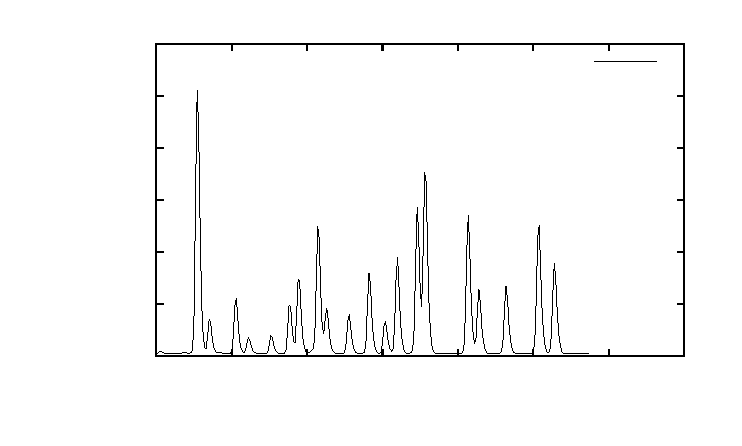
\includegraphics{ne-01}}%
    \gplfronttext
  \end{picture}%
\endgroup

			\caption{Spektrum der Neon-Glimmlampe betrachtet durch die mittlere Blende bei verwendetem Gitter mit $g = 200$, Belichtungszeit von 0.1 s und Temperatur von $0\unit{$^\circ$C}$}
			\label{ne_01}
		\end{figure}

		Vergleich mit dem im Anhang angegebenen Referenzspektrum zeigt nicht nur eine sehr gute Übereinstimmung der Lage der Spitzen von circa $580\unit{nm}$ bis $680\unit{nm}$ sondern auch noch eine sehr gute qualitative Ähnlichkeit der Intensität der Peaks mit denen der Referenz, da hier kein Papierfilter verwendet wurde.
		Auch in diesem Fall reicht die Auflösung des 200-Gitters völlig um alle Doppelpeaks klar trennen zu können, jedoch passt hier nicht mehr der gesamte Spektralbereich von $580\unit{nm}$ bis $750\unit{nm}$ auf eine Aufnahme.
	
	% subsection vergleichsspektren_von_hg_cd_und_ne (end)

	\subsection{Linearität der Dispersionsrelation} % (fold)
	\label{sub:linearit_t_der_dispersionsrelation}
	
		Verwendet man in Abbildung \ref{hg_01} die beiden äußeren Spektrallinien, welche nach Angabe der vorgegebenen Vergleichsspektren bei $435.8\unit{nm}$ und $643.8\unit{nm}$ zu finden sind, dann lassen sich die Skalierung $\alpha$ und das Offset $\beta$ bestimmen
		\begin{alignat*}{3}
			\alpha &= &0.35374\unit{nm} \\
			\beta &= &\ 414.2221\unit{nm}
		\end{alignat*}
		Durch diese Skalierung ergibt aus Abbildung \ref{hg_01} die Signalverteilung in Abhängigkeit der Wellenlänge (siehe).

		\begin{figure}
			\center
			% GNUPLOT: LaTeX picture with Postscript
\begingroup
  \makeatletter
  \providecommand\color[2][]{%
    \GenericError{(gnuplot) \space\space\space\@spaces}{%
      Package color not loaded in conjunction with
      terminal option `colourtext'%
    }{See the gnuplot documentation for explanation.%
    }{Either use 'blacktext' in gnuplot or load the package
      color.sty in LaTeX.}%
    \renewcommand\color[2][]{}%
  }%
  \providecommand\includegraphics[2][]{%
    \GenericError{(gnuplot) \space\space\space\@spaces}{%
      Package graphicx or graphics not loaded%
    }{See the gnuplot documentation for explanation.%
    }{The gnuplot epslatex terminal needs graphicx.sty or graphics.sty.}%
    \renewcommand\includegraphics[2][]{}%
  }%
  \providecommand\rotatebox[2]{#2}%
  \@ifundefined{ifGPcolor}{%
    \newif\ifGPcolor
    \GPcolorfalse
  }{}%
  \@ifundefined{ifGPblacktext}{%
    \newif\ifGPblacktext
    \GPblacktexttrue
  }{}%
  % define a \g@addto@macro without @ in the name:
  \let\gplgaddtomacro\g@addto@macro
  % define empty templates for all commands taking text:
  \gdef\gplbacktext{}%
  \gdef\gplfronttext{}%
  \makeatother
  \ifGPblacktext
    % no textcolor at all
    \def\colorrgb#1{}%
    \def\colorgray#1{}%
  \else
    % gray or color?
    \ifGPcolor
      \def\colorrgb#1{\color[rgb]{#1}}%
      \def\colorgray#1{\color[gray]{#1}}%
      \expandafter\def\csname LTw\endcsname{\color{white}}%
      \expandafter\def\csname LTb\endcsname{\color{black}}%
      \expandafter\def\csname LTa\endcsname{\color{black}}%
      \expandafter\def\csname LT0\endcsname{\color[rgb]{1,0,0}}%
      \expandafter\def\csname LT1\endcsname{\color[rgb]{0,1,0}}%
      \expandafter\def\csname LT2\endcsname{\color[rgb]{0,0,1}}%
      \expandafter\def\csname LT3\endcsname{\color[rgb]{1,0,1}}%
      \expandafter\def\csname LT4\endcsname{\color[rgb]{0,1,1}}%
      \expandafter\def\csname LT5\endcsname{\color[rgb]{1,1,0}}%
      \expandafter\def\csname LT6\endcsname{\color[rgb]{0,0,0}}%
      \expandafter\def\csname LT7\endcsname{\color[rgb]{1,0.3,0}}%
      \expandafter\def\csname LT8\endcsname{\color[rgb]{0.5,0.5,0.5}}%
    \else
      % gray
      \def\colorrgb#1{\color{black}}%
      \def\colorgray#1{\color[gray]{#1}}%
      \expandafter\def\csname LTw\endcsname{\color{white}}%
      \expandafter\def\csname LTb\endcsname{\color{black}}%
      \expandafter\def\csname LTa\endcsname{\color{black}}%
      \expandafter\def\csname LT0\endcsname{\color{black}}%
      \expandafter\def\csname LT1\endcsname{\color{black}}%
      \expandafter\def\csname LT2\endcsname{\color{black}}%
      \expandafter\def\csname LT3\endcsname{\color{black}}%
      \expandafter\def\csname LT4\endcsname{\color{black}}%
      \expandafter\def\csname LT5\endcsname{\color{black}}%
      \expandafter\def\csname LT6\endcsname{\color{black}}%
      \expandafter\def\csname LT7\endcsname{\color{black}}%
      \expandafter\def\csname LT8\endcsname{\color{black}}%
    \fi
  \fi
  \setlength{\unitlength}{0.0500bp}%
  \begin{picture}(6802.00,3968.00)%
    \gplgaddtomacro\gplbacktext{%
      \csname LTb\endcsname%
      \put(1078,704){\makebox(0,0)[r]{\strut{} 0}}%
      \put(1078,1132){\makebox(0,0)[r]{\strut{} 500}}%
      \put(1078,1561){\makebox(0,0)[r]{\strut{} 1000}}%
      \put(1078,1989){\makebox(0,0)[r]{\strut{} 1500}}%
      \put(1078,2418){\makebox(0,0)[r]{\strut{} 2000}}%
      \put(1078,2846){\makebox(0,0)[r]{\strut{} 2500}}%
      \put(1078,3275){\makebox(0,0)[r]{\strut{} 3000}}%
      \put(1078,3703){\makebox(0,0)[r]{\strut{} 3500}}%
      \put(1210,484){\makebox(0,0){\strut{} 400}}%
      \put(2076,484){\makebox(0,0){\strut{} 450}}%
      \put(2942,484){\makebox(0,0){\strut{} 500}}%
      \put(3808,484){\makebox(0,0){\strut{} 550}}%
      \put(4673,484){\makebox(0,0){\strut{} 600}}%
      \put(5539,484){\makebox(0,0){\strut{} 650}}%
      \put(6405,484){\makebox(0,0){\strut{} 700}}%
      \put(176,2203){\rotatebox{-270}{\makebox(0,0){\strut{}Intensität $I$}}}%
      \put(3807,154){\makebox(0,0){\strut{}Wellenlänge $\lambda \ [\unit{nm}]$}}%
    }%
    \gplgaddtomacro\gplfronttext{%
      \csname LTb\endcsname%
      \put(5418,3530){\makebox(0,0)[r]{\strut{}Messwerte}}%
    }%
    \gplbacktext
    \put(0,0){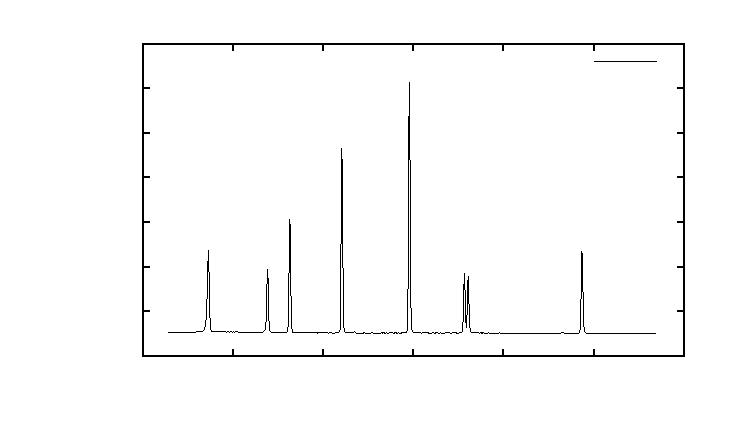
\includegraphics{hg-200-scale}}%
    \gplfronttext
  \end{picture}%
\endgroup

			\caption{Spektrum der Quecksilber-Cadmium-Entladungslampe über der Wellenlänge betrachtet durch die mittlere Blende bei verwendetem Gitter mit $g=200$, vorangestellten Papierfilter, Belichtungszeit von 0.1 s und Temperatur von $0\unit{$^\circ$C}$}
			\label{hg-scale}
		\end{figure}

		Die Linearität lässt sich nun durch Vergleich der gezeigten Wellenlängen mit den Bekannten überprüfen.
		Tabelle \ref{tab:hg-1} zeigt die typischen Spektrallinien für eine Hg-Cd-Lampe im Vergleich mit den gemessenen Werten.
		Die Fehlerwerte ergaben sich aus Ableseungenauigkeiten der Peak-Maxima.
		Innerhalb des untersuchten Bereiches kann die Dispersionsrelation im Rahmen der angegebenen Fehler als linear angenommen werden.

		\begin{table}
			\center
			\caption{Vergleich der gemessenen Spektrallinien und der Bekannten für die Hg-Cd-Lampe}
			\label{tab:hg-1}
			\begin{tabular}{c|c}
				Messwerte [nm] & Literaturwert [nm] \\
				\hline
				$469 \pm 2$ & 467.8 \\
				$481 \pm 2$ & 480.0 \\
				$510 \pm 2$ & 508.6 \\
				$547 \pm 2$ & 546.1 \\
				$577 \pm 2$ & 577.0 \\
				$580 \pm 2$ & 579.0 \\
			\end{tabular}
		\end{table}

	% subsection linearit_t_der_dispersionsrelation (end)

	\subsection{Auflösevermögen des Gitterspektrographen} % (fold)
	\label{sub:aufl_severm_gen_des_gitterspektrographen}

		Das Auflösungsvermögen lässt sich nun durch Ausmessen der halben Peak-Breite bestimmen.
		Als Beispiel sei hier der Peak bei $\lambda = 547\unit{nm}$ der Hg-Cd-Lampe aus \ref{hg-scale} angegeben.
		Dieser wurde durch die mittlere Spalte (und damit die schmalste) beleuchtet.
		Die gesamte Peak-Breite konnte zu $2\Delta \lambda = 3.9\unit{nm}$ bestimmt werden.
		\[ \frac{\lambda}{\Delta \lambda} \approx 281 \]
		Damit ist das Auflösungsvermögen weit unterhalb des zu erwartenden Auflösungsvermögen für ein Gitter, der sonst in Bereichen von ungefähr 2000 liegen müsste.
		Für das 200-Gitter ergaben sich dann je nach Spalt die in Tabelle \ref{tab:200-gitter-aufloesung} gezeigten Werte.

		\begin{table}
			\center
			\caption{Auflösungsvermögen des $547\unit{nm}$-Peaks der Hg-Cd-Lampe in Abhängigkeit der Spaltbreite am 200-Gitter}
			\label{tab:200-gitter-aufloesung}
			\begin{tabular}{r|r|r|r}
				Spaltbreite [$\mu$m] & 25 & 35 & 50 \\
				\hline
				Auflösungsvermögen & 281 & 257 & 205
			\end{tabular}
		\end{table}

		Um nun das 900-Gitter zu untersuchen ist in Abbildung \ref{hg-900-scale} das Spektrum der Hg-Cd-Lampe für das 900-Gitter im Bereich von $508\unit{nm}$ bis $580\unit{nm}$ gezeigt.
		Die Umrechnungskoeffizienten waren dabei
		\begin{alignat*}{3}
			\alpha &=& 0.0945\unit{nm} \\
			\beta &=& \ 507.2825\unit{nm}
		\end{alignat*}
		Für das Auflösungsvermögen ergeben sich dann analog die Werte aus Tabelle \ref{tab:900-gitter-aufloesung}.
		Es ist erkennbar, dass für das 900-Gitter ein wesentlich höheres Auflösungsvermögen erreicht wird.
		Dies ist auch mit der Theorie des Gitters zu vereinbaren, da die Spalte durch ein Lichtbündel konstanten Durchmessers beleuchtet werden.
		Es werden dadurch also sehr viel mehr Spalte beleuchtet als bei dem 200-Gitter.
		Das Auflösungsvermögen muss also verbessert werden.
		Dennoch liegt das gemessene Auflösungsvermögen weit unter einem theoretisch berechneten  Wert von ungefähr 10000.
		In den Grundlagen ist bereits beschrieben, dass dieses Problem durch eine endliche Spaltbreite entsteht.
		Wie erkennbar ist das Auflösungsvermögen also ebenfalls von der Spaltbreite abhängig. 

		\begin{figure}
			\center
			% GNUPLOT: LaTeX picture with Postscript
\begingroup
  \makeatletter
  \providecommand\color[2][]{%
    \GenericError{(gnuplot) \space\space\space\@spaces}{%
      Package color not loaded in conjunction with
      terminal option `colourtext'%
    }{See the gnuplot documentation for explanation.%
    }{Either use 'blacktext' in gnuplot or load the package
      color.sty in LaTeX.}%
    \renewcommand\color[2][]{}%
  }%
  \providecommand\includegraphics[2][]{%
    \GenericError{(gnuplot) \space\space\space\@spaces}{%
      Package graphicx or graphics not loaded%
    }{See the gnuplot documentation for explanation.%
    }{The gnuplot epslatex terminal needs graphicx.sty or graphics.sty.}%
    \renewcommand\includegraphics[2][]{}%
  }%
  \providecommand\rotatebox[2]{#2}%
  \@ifundefined{ifGPcolor}{%
    \newif\ifGPcolor
    \GPcolorfalse
  }{}%
  \@ifundefined{ifGPblacktext}{%
    \newif\ifGPblacktext
    \GPblacktexttrue
  }{}%
  % define a \g@addto@macro without @ in the name:
  \let\gplgaddtomacro\g@addto@macro
  % define empty templates for all commands taking text:
  \gdef\gplbacktext{}%
  \gdef\gplfronttext{}%
  \makeatother
  \ifGPblacktext
    % no textcolor at all
    \def\colorrgb#1{}%
    \def\colorgray#1{}%
  \else
    % gray or color?
    \ifGPcolor
      \def\colorrgb#1{\color[rgb]{#1}}%
      \def\colorgray#1{\color[gray]{#1}}%
      \expandafter\def\csname LTw\endcsname{\color{white}}%
      \expandafter\def\csname LTb\endcsname{\color{black}}%
      \expandafter\def\csname LTa\endcsname{\color{black}}%
      \expandafter\def\csname LT0\endcsname{\color[rgb]{1,0,0}}%
      \expandafter\def\csname LT1\endcsname{\color[rgb]{0,1,0}}%
      \expandafter\def\csname LT2\endcsname{\color[rgb]{0,0,1}}%
      \expandafter\def\csname LT3\endcsname{\color[rgb]{1,0,1}}%
      \expandafter\def\csname LT4\endcsname{\color[rgb]{0,1,1}}%
      \expandafter\def\csname LT5\endcsname{\color[rgb]{1,1,0}}%
      \expandafter\def\csname LT6\endcsname{\color[rgb]{0,0,0}}%
      \expandafter\def\csname LT7\endcsname{\color[rgb]{1,0.3,0}}%
      \expandafter\def\csname LT8\endcsname{\color[rgb]{0.5,0.5,0.5}}%
    \else
      % gray
      \def\colorrgb#1{\color{black}}%
      \def\colorgray#1{\color[gray]{#1}}%
      \expandafter\def\csname LTw\endcsname{\color{white}}%
      \expandafter\def\csname LTb\endcsname{\color{black}}%
      \expandafter\def\csname LTa\endcsname{\color{black}}%
      \expandafter\def\csname LT0\endcsname{\color{black}}%
      \expandafter\def\csname LT1\endcsname{\color{black}}%
      \expandafter\def\csname LT2\endcsname{\color{black}}%
      \expandafter\def\csname LT3\endcsname{\color{black}}%
      \expandafter\def\csname LT4\endcsname{\color{black}}%
      \expandafter\def\csname LT5\endcsname{\color{black}}%
      \expandafter\def\csname LT6\endcsname{\color{black}}%
      \expandafter\def\csname LT7\endcsname{\color{black}}%
      \expandafter\def\csname LT8\endcsname{\color{black}}%
    \fi
  \fi
  \setlength{\unitlength}{0.0500bp}%
  \begin{picture}(6802.00,3968.00)%
    \gplgaddtomacro\gplbacktext{%
      \csname LTb\endcsname%
      \put(1210,704){\makebox(0,0)[r]{\strut{} 0}}%
      \put(1210,1204){\makebox(0,0)[r]{\strut{} 5000}}%
      \put(1210,1704){\makebox(0,0)[r]{\strut{} 10000}}%
      \put(1210,2204){\makebox(0,0)[r]{\strut{} 15000}}%
      \put(1210,2703){\makebox(0,0)[r]{\strut{} 20000}}%
      \put(1210,3203){\makebox(0,0)[r]{\strut{} 25000}}%
      \put(1210,3703){\makebox(0,0)[r]{\strut{} 30000}}%
      \put(1342,484){\makebox(0,0){\strut{} 500}}%
      \put(1975,484){\makebox(0,0){\strut{} 510}}%
      \put(2608,484){\makebox(0,0){\strut{} 520}}%
      \put(3241,484){\makebox(0,0){\strut{} 530}}%
      \put(3874,484){\makebox(0,0){\strut{} 540}}%
      \put(4506,484){\makebox(0,0){\strut{} 550}}%
      \put(5139,484){\makebox(0,0){\strut{} 560}}%
      \put(5772,484){\makebox(0,0){\strut{} 570}}%
      \put(6405,484){\makebox(0,0){\strut{} 580}}%
      \put(176,2203){\rotatebox{-270}{\makebox(0,0){\strut{}Intensität $I$}}}%
      \put(3873,154){\makebox(0,0){\strut{}Wellenlänge $\lambda \ [\mathrm{nm}]$}}%
    }%
    \gplgaddtomacro\gplfronttext{%
      \csname LTb\endcsname%
      \put(5418,3530){\makebox(0,0)[r]{\strut{}Messwerte}}%
    }%
    \gplbacktext
    \put(0,0){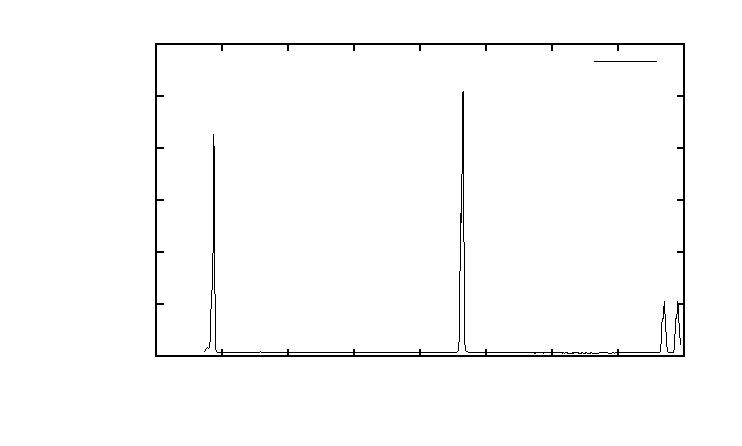
\includegraphics{hg-900-scale-1}}%
    \gplfronttext
  \end{picture}%
\endgroup

			\caption{Spektrum der Quecksilber-Cadmium-Entladungslampe über der Wellenlänge betrachtet durch die mittlere Blende bei verwendetem Gitter mit $g=900$, vorangestellten Papierfilter, Belichtungszeit von 0.1 s und Temperatur von $0\unit{$^\circ$C}$}
			\label{hg-900-scale}
		\end{figure}

		\begin{table}
			\center
			\caption{Auflösungsvermögen des $547\unit{nm}$-Peaks der Hg-Cd-Lampe in Abhängigkeit der Spaltbreite am 900-Gitter}
			\label{tab:900-gitter-aufloesung}
			\begin{tabular}{r|r|r|r}
				Spaltbreite [$\mu$m] & 25 & 35 & 50 \\
				\hline
				Auflösungsvermögen & 890 & 772 & 681
			\end{tabular}
		\end{table}

	% subsection aufl_severm_gen_des_gitterspektrographen (end)

	\subsection{Spektren des Sonnenlichts} % (fold)
	\label{sub:spektren_des_sonnenlichts}

		Die Sonnenspektren wurden, wie in der Durchführung beschrieben, aufgenommen und mit dem im Anschluss erstellten Vergleichsspektren kalibriert und skaliert.
		Um ein bestmögliches Auflösungsvermögen zu erreichen verwendeten wir im Folgenden für alle Messungen das 900-Gitter und den mittleren und damit auch den schmalsten Spalt.
		Die Temperatur des CCD-Sensors betrug immer $0\unit{$^\circ$C}$ und die Belichtungszeit $1\unit{s}$.

		\begin{figure}
			\center
			% GNUPLOT: LaTeX picture with Postscript
\begingroup
  \makeatletter
  \providecommand\color[2][]{%
    \GenericError{(gnuplot) \space\space\space\@spaces}{%
      Package color not loaded in conjunction with
      terminal option `colourtext'%
    }{See the gnuplot documentation for explanation.%
    }{Either use 'blacktext' in gnuplot or load the package
      color.sty in LaTeX.}%
    \renewcommand\color[2][]{}%
  }%
  \providecommand\includegraphics[2][]{%
    \GenericError{(gnuplot) \space\space\space\@spaces}{%
      Package graphicx or graphics not loaded%
    }{See the gnuplot documentation for explanation.%
    }{The gnuplot epslatex terminal needs graphicx.sty or graphics.sty.}%
    \renewcommand\includegraphics[2][]{}%
  }%
  \providecommand\rotatebox[2]{#2}%
  \@ifundefined{ifGPcolor}{%
    \newif\ifGPcolor
    \GPcolorfalse
  }{}%
  \@ifundefined{ifGPblacktext}{%
    \newif\ifGPblacktext
    \GPblacktexttrue
  }{}%
  % define a \g@addto@macro without @ in the name:
  \let\gplgaddtomacro\g@addto@macro
  % define empty templates for all commands taking text:
  \gdef\gplbacktext{}%
  \gdef\gplfronttext{}%
  \makeatother
  \ifGPblacktext
    % no textcolor at all
    \def\colorrgb#1{}%
    \def\colorgray#1{}%
  \else
    % gray or color?
    \ifGPcolor
      \def\colorrgb#1{\color[rgb]{#1}}%
      \def\colorgray#1{\color[gray]{#1}}%
      \expandafter\def\csname LTw\endcsname{\color{white}}%
      \expandafter\def\csname LTb\endcsname{\color{black}}%
      \expandafter\def\csname LTa\endcsname{\color{black}}%
      \expandafter\def\csname LT0\endcsname{\color[rgb]{1,0,0}}%
      \expandafter\def\csname LT1\endcsname{\color[rgb]{0,1,0}}%
      \expandafter\def\csname LT2\endcsname{\color[rgb]{0,0,1}}%
      \expandafter\def\csname LT3\endcsname{\color[rgb]{1,0,1}}%
      \expandafter\def\csname LT4\endcsname{\color[rgb]{0,1,1}}%
      \expandafter\def\csname LT5\endcsname{\color[rgb]{1,1,0}}%
      \expandafter\def\csname LT6\endcsname{\color[rgb]{0,0,0}}%
      \expandafter\def\csname LT7\endcsname{\color[rgb]{1,0.3,0}}%
      \expandafter\def\csname LT8\endcsname{\color[rgb]{0.5,0.5,0.5}}%
    \else
      % gray
      \def\colorrgb#1{\color{black}}%
      \def\colorgray#1{\color[gray]{#1}}%
      \expandafter\def\csname LTw\endcsname{\color{white}}%
      \expandafter\def\csname LTb\endcsname{\color{black}}%
      \expandafter\def\csname LTa\endcsname{\color{black}}%
      \expandafter\def\csname LT0\endcsname{\color{black}}%
      \expandafter\def\csname LT1\endcsname{\color{black}}%
      \expandafter\def\csname LT2\endcsname{\color{black}}%
      \expandafter\def\csname LT3\endcsname{\color{black}}%
      \expandafter\def\csname LT4\endcsname{\color{black}}%
      \expandafter\def\csname LT5\endcsname{\color{black}}%
      \expandafter\def\csname LT6\endcsname{\color{black}}%
      \expandafter\def\csname LT7\endcsname{\color{black}}%
      \expandafter\def\csname LT8\endcsname{\color{black}}%
    \fi
  \fi
  \setlength{\unitlength}{0.0500bp}%
  \begin{picture}(6802.00,3968.00)%
    \gplgaddtomacro\gplbacktext{%
      \csname LTb\endcsname%
      \put(1078,704){\makebox(0,0)[r]{\strut{} 800}}%
      \put(1078,1037){\makebox(0,0)[r]{\strut{} 850}}%
      \put(1078,1370){\makebox(0,0)[r]{\strut{} 900}}%
      \put(1078,1704){\makebox(0,0)[r]{\strut{} 950}}%
      \put(1078,2037){\makebox(0,0)[r]{\strut{} 1000}}%
      \put(1078,2370){\makebox(0,0)[r]{\strut{} 1050}}%
      \put(1078,2703){\makebox(0,0)[r]{\strut{} 1100}}%
      \put(1078,3037){\makebox(0,0)[r]{\strut{} 1150}}%
      \put(1078,3370){\makebox(0,0)[r]{\strut{} 1200}}%
      \put(1078,3703){\makebox(0,0)[r]{\strut{} 1250}}%
      \put(1210,484){\makebox(0,0){\strut{} 500}}%
      \put(1859,484){\makebox(0,0){\strut{} 510}}%
      \put(2509,484){\makebox(0,0){\strut{} 520}}%
      \put(3158,484){\makebox(0,0){\strut{} 530}}%
      \put(3808,484){\makebox(0,0){\strut{} 540}}%
      \put(4457,484){\makebox(0,0){\strut{} 550}}%
      \put(5106,484){\makebox(0,0){\strut{} 560}}%
      \put(5756,484){\makebox(0,0){\strut{} 570}}%
      \put(6405,484){\makebox(0,0){\strut{} 580}}%
      \put(176,2203){\rotatebox{-270}{\makebox(0,0){\strut{}Intensität $I$}}}%
      \put(3807,154){\makebox(0,0){\strut{}Wellenlänge $\lambda \ [\unit{nm}]$}}%
    }%
    \gplgaddtomacro\gplfronttext{%
      \csname LTb\endcsname%
      \put(5418,3530){\makebox(0,0)[r]{\strut{}Messwerte}}%
    }%
    \gplbacktext
    \put(0,0){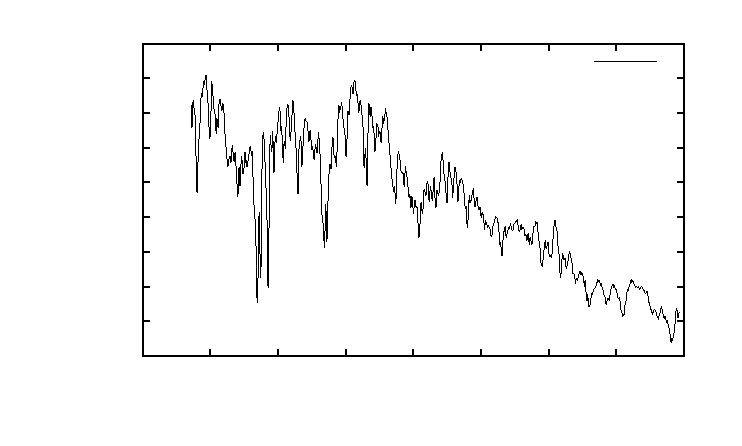
\includegraphics{sonne-p1}}%
    \gplfronttext
  \end{picture}%
\endgroup

			\caption{gemessenes Spektrum des natürlichen Lichts}
			\label{sonne-p1}
		\end{figure}

		\begin{figure}
			\center
			% GNUPLOT: LaTeX picture with Postscript
\begingroup
  \makeatletter
  \providecommand\color[2][]{%
    \GenericError{(gnuplot) \space\space\space\@spaces}{%
      Package color not loaded in conjunction with
      terminal option `colourtext'%
    }{See the gnuplot documentation for explanation.%
    }{Either use 'blacktext' in gnuplot or load the package
      color.sty in LaTeX.}%
    \renewcommand\color[2][]{}%
  }%
  \providecommand\includegraphics[2][]{%
    \GenericError{(gnuplot) \space\space\space\@spaces}{%
      Package graphicx or graphics not loaded%
    }{See the gnuplot documentation for explanation.%
    }{The gnuplot epslatex terminal needs graphicx.sty or graphics.sty.}%
    \renewcommand\includegraphics[2][]{}%
  }%
  \providecommand\rotatebox[2]{#2}%
  \@ifundefined{ifGPcolor}{%
    \newif\ifGPcolor
    \GPcolorfalse
  }{}%
  \@ifundefined{ifGPblacktext}{%
    \newif\ifGPblacktext
    \GPblacktexttrue
  }{}%
  % define a \g@addto@macro without @ in the name:
  \let\gplgaddtomacro\g@addto@macro
  % define empty templates for all commands taking text:
  \gdef\gplbacktext{}%
  \gdef\gplfronttext{}%
  \makeatother
  \ifGPblacktext
    % no textcolor at all
    \def\colorrgb#1{}%
    \def\colorgray#1{}%
  \else
    % gray or color?
    \ifGPcolor
      \def\colorrgb#1{\color[rgb]{#1}}%
      \def\colorgray#1{\color[gray]{#1}}%
      \expandafter\def\csname LTw\endcsname{\color{white}}%
      \expandafter\def\csname LTb\endcsname{\color{black}}%
      \expandafter\def\csname LTa\endcsname{\color{black}}%
      \expandafter\def\csname LT0\endcsname{\color[rgb]{1,0,0}}%
      \expandafter\def\csname LT1\endcsname{\color[rgb]{0,1,0}}%
      \expandafter\def\csname LT2\endcsname{\color[rgb]{0,0,1}}%
      \expandafter\def\csname LT3\endcsname{\color[rgb]{1,0,1}}%
      \expandafter\def\csname LT4\endcsname{\color[rgb]{0,1,1}}%
      \expandafter\def\csname LT5\endcsname{\color[rgb]{1,1,0}}%
      \expandafter\def\csname LT6\endcsname{\color[rgb]{0,0,0}}%
      \expandafter\def\csname LT7\endcsname{\color[rgb]{1,0.3,0}}%
      \expandafter\def\csname LT8\endcsname{\color[rgb]{0.5,0.5,0.5}}%
    \else
      % gray
      \def\colorrgb#1{\color{black}}%
      \def\colorgray#1{\color[gray]{#1}}%
      \expandafter\def\csname LTw\endcsname{\color{white}}%
      \expandafter\def\csname LTb\endcsname{\color{black}}%
      \expandafter\def\csname LTa\endcsname{\color{black}}%
      \expandafter\def\csname LT0\endcsname{\color{black}}%
      \expandafter\def\csname LT1\endcsname{\color{black}}%
      \expandafter\def\csname LT2\endcsname{\color{black}}%
      \expandafter\def\csname LT3\endcsname{\color{black}}%
      \expandafter\def\csname LT4\endcsname{\color{black}}%
      \expandafter\def\csname LT5\endcsname{\color{black}}%
      \expandafter\def\csname LT6\endcsname{\color{black}}%
      \expandafter\def\csname LT7\endcsname{\color{black}}%
      \expandafter\def\csname LT8\endcsname{\color{black}}%
    \fi
  \fi
  \setlength{\unitlength}{0.0500bp}%
  \begin{picture}(6802.00,3968.00)%
    \gplgaddtomacro\gplbacktext{%
      \csname LTb\endcsname%
      \put(1078,704){\makebox(0,0)[r]{\strut{} 650}}%
      \put(1078,1132){\makebox(0,0)[r]{\strut{} 700}}%
      \put(1078,1561){\makebox(0,0)[r]{\strut{} 750}}%
      \put(1078,1989){\makebox(0,0)[r]{\strut{} 800}}%
      \put(1078,2418){\makebox(0,0)[r]{\strut{} 850}}%
      \put(1078,2846){\makebox(0,0)[r]{\strut{} 900}}%
      \put(1078,3275){\makebox(0,0)[r]{\strut{} 950}}%
      \put(1078,3703){\makebox(0,0)[r]{\strut{} 1000}}%
      \put(1210,484){\makebox(0,0){\strut{} 570}}%
      \put(1952,484){\makebox(0,0){\strut{} 580}}%
      \put(2694,484){\makebox(0,0){\strut{} 590}}%
      \put(3436,484){\makebox(0,0){\strut{} 600}}%
      \put(4179,484){\makebox(0,0){\strut{} 610}}%
      \put(4921,484){\makebox(0,0){\strut{} 620}}%
      \put(5663,484){\makebox(0,0){\strut{} 630}}%
      \put(6405,484){\makebox(0,0){\strut{} 640}}%
      \put(176,2203){\rotatebox{-270}{\makebox(0,0){\strut{}Intensität $I$}}}%
      \put(3807,154){\makebox(0,0){\strut{}Wellenlänge $\lambda \ [\unit{nm}]$}}%
    }%
    \gplgaddtomacro\gplfronttext{%
      \csname LTb\endcsname%
      \put(5418,3530){\makebox(0,0)[r]{\strut{}Messwerte}}%
    }%
    \gplbacktext
    \put(0,0){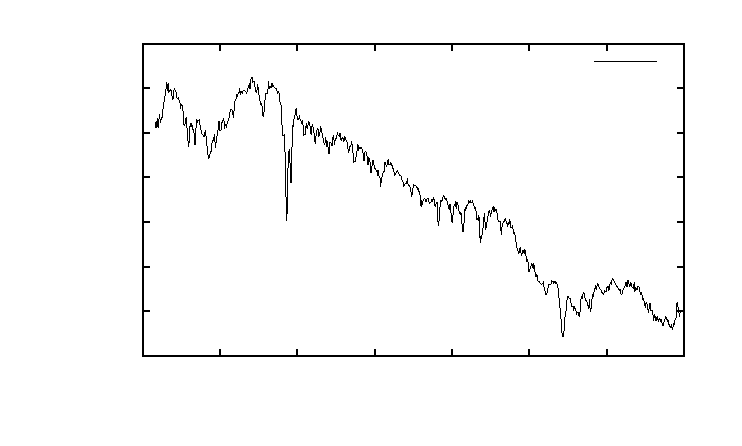
\includegraphics{sonne-p2}}%
    \gplfronttext
  \end{picture}%
\endgroup

			\caption{gemessenes Spektrum des natürlichen Lichts}
			\label{sonne-p2}
		\end{figure}

		\begin{figure}
			\center
			% GNUPLOT: LaTeX picture with Postscript
\begingroup
  \makeatletter
  \providecommand\color[2][]{%
    \GenericError{(gnuplot) \space\space\space\@spaces}{%
      Package color not loaded in conjunction with
      terminal option `colourtext'%
    }{See the gnuplot documentation for explanation.%
    }{Either use 'blacktext' in gnuplot or load the package
      color.sty in LaTeX.}%
    \renewcommand\color[2][]{}%
  }%
  \providecommand\includegraphics[2][]{%
    \GenericError{(gnuplot) \space\space\space\@spaces}{%
      Package graphicx or graphics not loaded%
    }{See the gnuplot documentation for explanation.%
    }{The gnuplot epslatex terminal needs graphicx.sty or graphics.sty.}%
    \renewcommand\includegraphics[2][]{}%
  }%
  \providecommand\rotatebox[2]{#2}%
  \@ifundefined{ifGPcolor}{%
    \newif\ifGPcolor
    \GPcolorfalse
  }{}%
  \@ifundefined{ifGPblacktext}{%
    \newif\ifGPblacktext
    \GPblacktexttrue
  }{}%
  % define a \g@addto@macro without @ in the name:
  \let\gplgaddtomacro\g@addto@macro
  % define empty templates for all commands taking text:
  \gdef\gplbacktext{}%
  \gdef\gplfronttext{}%
  \makeatother
  \ifGPblacktext
    % no textcolor at all
    \def\colorrgb#1{}%
    \def\colorgray#1{}%
  \else
    % gray or color?
    \ifGPcolor
      \def\colorrgb#1{\color[rgb]{#1}}%
      \def\colorgray#1{\color[gray]{#1}}%
      \expandafter\def\csname LTw\endcsname{\color{white}}%
      \expandafter\def\csname LTb\endcsname{\color{black}}%
      \expandafter\def\csname LTa\endcsname{\color{black}}%
      \expandafter\def\csname LT0\endcsname{\color[rgb]{1,0,0}}%
      \expandafter\def\csname LT1\endcsname{\color[rgb]{0,1,0}}%
      \expandafter\def\csname LT2\endcsname{\color[rgb]{0,0,1}}%
      \expandafter\def\csname LT3\endcsname{\color[rgb]{1,0,1}}%
      \expandafter\def\csname LT4\endcsname{\color[rgb]{0,1,1}}%
      \expandafter\def\csname LT5\endcsname{\color[rgb]{1,1,0}}%
      \expandafter\def\csname LT6\endcsname{\color[rgb]{0,0,0}}%
      \expandafter\def\csname LT7\endcsname{\color[rgb]{1,0.3,0}}%
      \expandafter\def\csname LT8\endcsname{\color[rgb]{0.5,0.5,0.5}}%
    \else
      % gray
      \def\colorrgb#1{\color{black}}%
      \def\colorgray#1{\color[gray]{#1}}%
      \expandafter\def\csname LTw\endcsname{\color{white}}%
      \expandafter\def\csname LTb\endcsname{\color{black}}%
      \expandafter\def\csname LTa\endcsname{\color{black}}%
      \expandafter\def\csname LT0\endcsname{\color{black}}%
      \expandafter\def\csname LT1\endcsname{\color{black}}%
      \expandafter\def\csname LT2\endcsname{\color{black}}%
      \expandafter\def\csname LT3\endcsname{\color{black}}%
      \expandafter\def\csname LT4\endcsname{\color{black}}%
      \expandafter\def\csname LT5\endcsname{\color{black}}%
      \expandafter\def\csname LT6\endcsname{\color{black}}%
      \expandafter\def\csname LT7\endcsname{\color{black}}%
      \expandafter\def\csname LT8\endcsname{\color{black}}%
    \fi
  \fi
  \setlength{\unitlength}{0.0500bp}%
  \begin{picture}(6802.00,3968.00)%
    \gplgaddtomacro\gplbacktext{%
      \csname LTb\endcsname%
      \put(946,704){\makebox(0,0)[r]{\strut{} 400}}%
      \put(946,1079){\makebox(0,0)[r]{\strut{} 450}}%
      \put(946,1454){\makebox(0,0)[r]{\strut{} 500}}%
      \put(946,1829){\makebox(0,0)[r]{\strut{} 550}}%
      \put(946,2204){\makebox(0,0)[r]{\strut{} 600}}%
      \put(946,2578){\makebox(0,0)[r]{\strut{} 650}}%
      \put(946,2953){\makebox(0,0)[r]{\strut{} 700}}%
      \put(946,3328){\makebox(0,0)[r]{\strut{} 750}}%
      \put(946,3703){\makebox(0,0)[r]{\strut{} 800}}%
      \put(1078,484){\makebox(0,0){\strut{} 620}}%
      \put(1744,484){\makebox(0,0){\strut{} 630}}%
      \put(2410,484){\makebox(0,0){\strut{} 640}}%
      \put(3076,484){\makebox(0,0){\strut{} 650}}%
      \put(3742,484){\makebox(0,0){\strut{} 660}}%
      \put(4407,484){\makebox(0,0){\strut{} 670}}%
      \put(5073,484){\makebox(0,0){\strut{} 680}}%
      \put(5739,484){\makebox(0,0){\strut{} 690}}%
      \put(6405,484){\makebox(0,0){\strut{} 700}}%
      \put(176,2203){\rotatebox{-270}{\makebox(0,0){\strut{}Intensität $I$}}}%
      \put(3741,154){\makebox(0,0){\strut{}Wellenlänge $\lambda \ [\unit{nm}]$}}%
    }%
    \gplgaddtomacro\gplfronttext{%
      \csname LTb\endcsname%
      \put(5418,3530){\makebox(0,0)[r]{\strut{}Messwerte}}%
    }%
    \gplbacktext
    \put(0,0){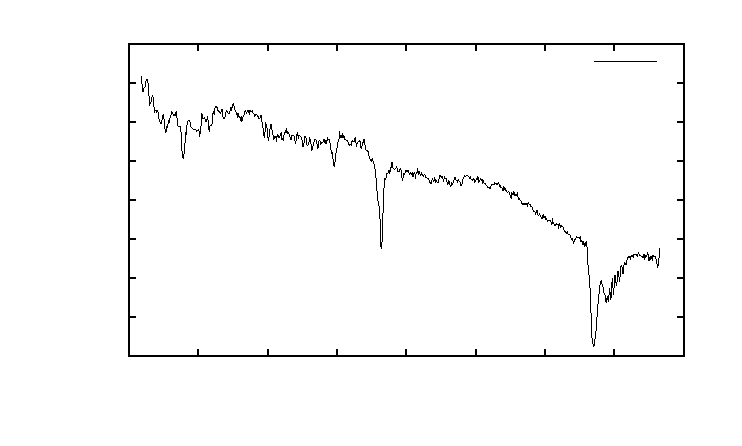
\includegraphics{sonne-p3}}%
    \gplfronttext
  \end{picture}%
\endgroup

			\caption{gemessenes Spektrum des natürlichen Lichts}
			\label{sonne-p3}
		\end{figure}

		In den Abbildungen \ref{sonne-p1}, \ref{sonne-p2} und \ref{sonne-p3} lassen sich nun charakteristische Absorptionslinien herauslesen. 
		Diese sind in Tabelle \ref{tab:sonne-spec} aufgeführt.
		Durch die im Anhang angegebenen Sonnenspektren konnten alle Linien nachvollzogen werden.
		Es konnte eine sehr gute Übereinstimmung mit den angegebenen Werten erreicht werden, wodurch auch verschiedene Elemente in Sonne und Atmosphäre nachgewiesen werden konnten.

		\begin{table}
			\center
			\caption{gemessene Absorptionslinien des natürlichen Lichts mit zugeordneten Elementen und Linien}
			\label{tab:sonne-spec}
			\begin{tabular}{c|r}
				Messwerte [nm] & Linie/Element \\
				\hline
				517 & MgI \\
				518 & MgI \\
				525 & FeI \\
				540 & FeI \\
				578 & CaI \\
				588 & Na \\
				624 & O$_2$(tell.) \\
				656 & H$\alpha$ \\
				686 & O$_2$(tell.)
			\end{tabular}
		\end{table}
	
	% subsection spektren_des_sonnenlichts (end)
% section messwerte_und_auswertung (end)